%%  本模板推荐以下方式编译: xelatex
%%     1. 文件默认的编码为 UTF-8 对于windows,请选用支持UTF-8编码的编辑器。
%%   2. 若是模板有什么问题,请及时与我们取得联系,Email:latexstudio@qq.com。
%%   3. 可以到  https://ask.latexstudio.net 提问
%%   4. 请安装 最新版本的 TeXLive 地址:
%%   http://mirrors.ctan.org/systems/texlive/Images/texlive.iso

\documentclass[12pt,a4paper]{nmmcm}
\usepackage{ctex}
\usepackage{gbt7714}
\usepackage{float}
\usepackage{graphicx}
\usepackage{booktabs,colortbl}
\usepackage{xcolor}
\usepackage{tikz}
\usepackage{indentfirst}
\mcmsetup{CTeX = true,
        tcn ={\xiaowuhao 1001 }(\textcolor{red}{\textit{1103}}), problem = A,
        sheet = true, titleinsheet = false, keywordsinsheet = true,
        titlepage = true, abstract = true}
\usepackage{xurl}
\setmainfont{Times New Roman}
\setmonofont[
    Path=fonts/,
    UprightFont = *-Regular,
    BoldFont = *-Bold,
    ItalicFont = *-Italic
]{UbuntuMono}
\usepackage{lipsum}


\usepackage{paralist}
\let\itemize\compactitem
\let\enditemize\endcompactitem
\let\enumerate\compactenum
\let\endenumerate\endcompactenum
\let\description\compactdesc
\let\enddescription\endcompactdesc

\setlength{\parindent}{2em} 
\setlength\abovedisplayskip{5pt}
\setlength\belowdisplayskip{-8pt}
\setlength{\parskip}{0.1em}

\newcommand\wordc[1]{\textbf{#1}}
\renewcommand{\appendixtocname}{附\quad录}
\renewcommand{\appendices}{\hspace{-2em}{\sanhao\HEI {\bf 附~~~录}}}
\colorlet{tableheadcolor}{gray!25} % Table header colour = 25% gray
\newcommand{\headcol}{\rowcolor{tableheadcolor}}

\title{TRS}
\date{}

\usepackage[font=small,labelfont={bf,sf},tableposition=top]{caption}


\begin{document}
\begin{abstract}


%abstract---------------
{\fangsong\xiaosihao
\setlength{\parindent}{2em}
社会消费品零售总额是衡量人们消费水平的重要指标,也是国民经济体系中的一个重要指标。
预测2022年疫情损失的社会消费品零售总额,可以将其应用于的对整体经济损失的一个关键要素。

首先通过对以往月度统计数据进行STL季节性分解,得到时间序列的季节波动情况。
然后先对原时间序列进行一阶差分,再对差分后序列进行季节差分,得到平稳的时间序列。再通过季节性ARIMA模型进行参数估计,并
得到2022年未受到疫情干预的预测值。接着利用2020年前的数据建立ARIMA模型,得到2020年未受疫情影响的预测值。通过2020年
预测值和实际值,建立在疫情干预下的干预分析模型。继而应用该模型得到2022年在疫情干预下的
预测值。最终结合ARIMA模型的预测值,预测2022年社会消费品零售总额的损失。
并通过R语言进行建模和计算以及绘图。
}









\begin{keywords}
{\song\xiaosihao
社会消费品零售总额,ARIMA,时间序列分析}
\end{keywords}


\end{abstract}
\maketitle
\renewcommand{\contentsname}{\centerline{\sanhao\bfseries\HEI 目\quad 录}}
%\thispagestyle{empty}
%{\song\xiaosihao
\tableofcontents
%}

\newpage
\setcounter{page}{1}
\pagestyle{fancy}
\song\xiaosihao
\section{数据分析}
\subsection{数据来源}
tess
本次建模采用的数据为2012年1月起至2022年3月的月度数据,\href{http://www.gov.cn/shuju/hgjjyxqk/xiangqing/tcg.html}{来自国家统计局}。
由于在 1-2 月只有总和的数据,在此简单假设两月每天的零售总额相同,
则一月份总额在 1-2 月总和的占比在闰年和平年的占比分别为
\(51.7\% \; ,52.5\%\) ,得到表格如下:
% Table generated by Excel2LaTeX from sheet 'Sheet1'
\begin{table}[htb]
  \centering
  \caption{社会商品零售总额月度数据(单位: 亿元)}
  \resizebox{\textwidth}{!}{
    \begin{tabular}{c|ccccccccccc}
          & 2012  & 2013  & 2014  & 2015  & 2016  & 2017  & 2018  & 2019  & 2020  & 2021  & 2022 \\
          \hline
    1     & 17171.0  & 19866.4  & 21563.2  & 25216.7  & 26984.3  & 30453.8  & 31151.7  & 34712.0  & 27390.6  & 36641.8  & 37957.3  \\
    2     & 16497.6  & 17943.4  & 20717.5  & 22775.8  & 25926.0  & 27505.9  & 29930.1  & 31352.0  & 24739.2  & 33095.0  & 36468.7  \\
    3     & 15650.2 & 17641.2 & 19800.6 & 22722.8 & 25114.1 & 27863.7 & 29193.6 & 31725.7 & 26449.9 & 35484.1 & 34233.1 \\
    4     & 15603.1 & 17600.3 & 19701.2 & 22386.7 & 24645.8 & 27278.5 & 28541.9 & 30586.1 & 28177.8 & 33152.6 &  \\
    5     & 16714.8 & 18886.3 & 21249.8 & 24194.8 & 26610.7 & 29459.2 & 30359.1 & 32955.7 & 31972.8 & 35945.1 &  \\
    6     & 16584.9 & 18826.7 & 21166.4 & 24280.3 & 26857.4 & 29807.6 & 30841.6 & 33878.1 & 33525.9 & 37585.8 &  \\
    7     & 16314.9 & 18513.2 & 20775.8 & 24338.8 & 26827.4 & 29609.8 & 30733.7 & 33073.3 & 32202.5 & 34925.1 &  \\
    8     & 16658.9 & 18886.2 & 21133.9 & 24893.4 & 27539.6 & 30329.7 & 31542.3 & 33896.3 & 33570.6 & 34394.9 &  \\
    9     & 18226.6 & 20653.3 & 23042.4 & 25270.6 & 27976.4 & 30870.3 & 32005.4 & 34494.9 & 35294.7 & 36833.0 &  \\
    10    & 18933.8 & 21491.3 & 23967.2 & 28278.9 & 31119.2 & 34240.9 & 35534.4 & 38104.3 & 38576.5 & 40453.9 &  \\
    11    & 18476.7 & 21011.9 & 23474.7 & 27937.3 & 30958.5 & 34108.2 & 35259.7 & 38093.8 & 39514.2 & 41043.2 &  \\
    12    & 20334.2 & 23059.7 & 25801.3 & 28634.6 & 31757.0 & 34734.1 & 35893.5 & 38776.7 & 40566.0 & 41268.9 &  \\
    \end{tabular}}%
  \label{tab:addlabel}%
\end{table}%

根据表格中所给数据,选择2022年1,2,3月作为测试集,剩余数据作为训练集,以时间为横轴,绘出折线图如下:
\begin{figure}[H] %H为当前位置,!htb为忽略美学标准,htbp为浮动图形
  \centering %图片居中
  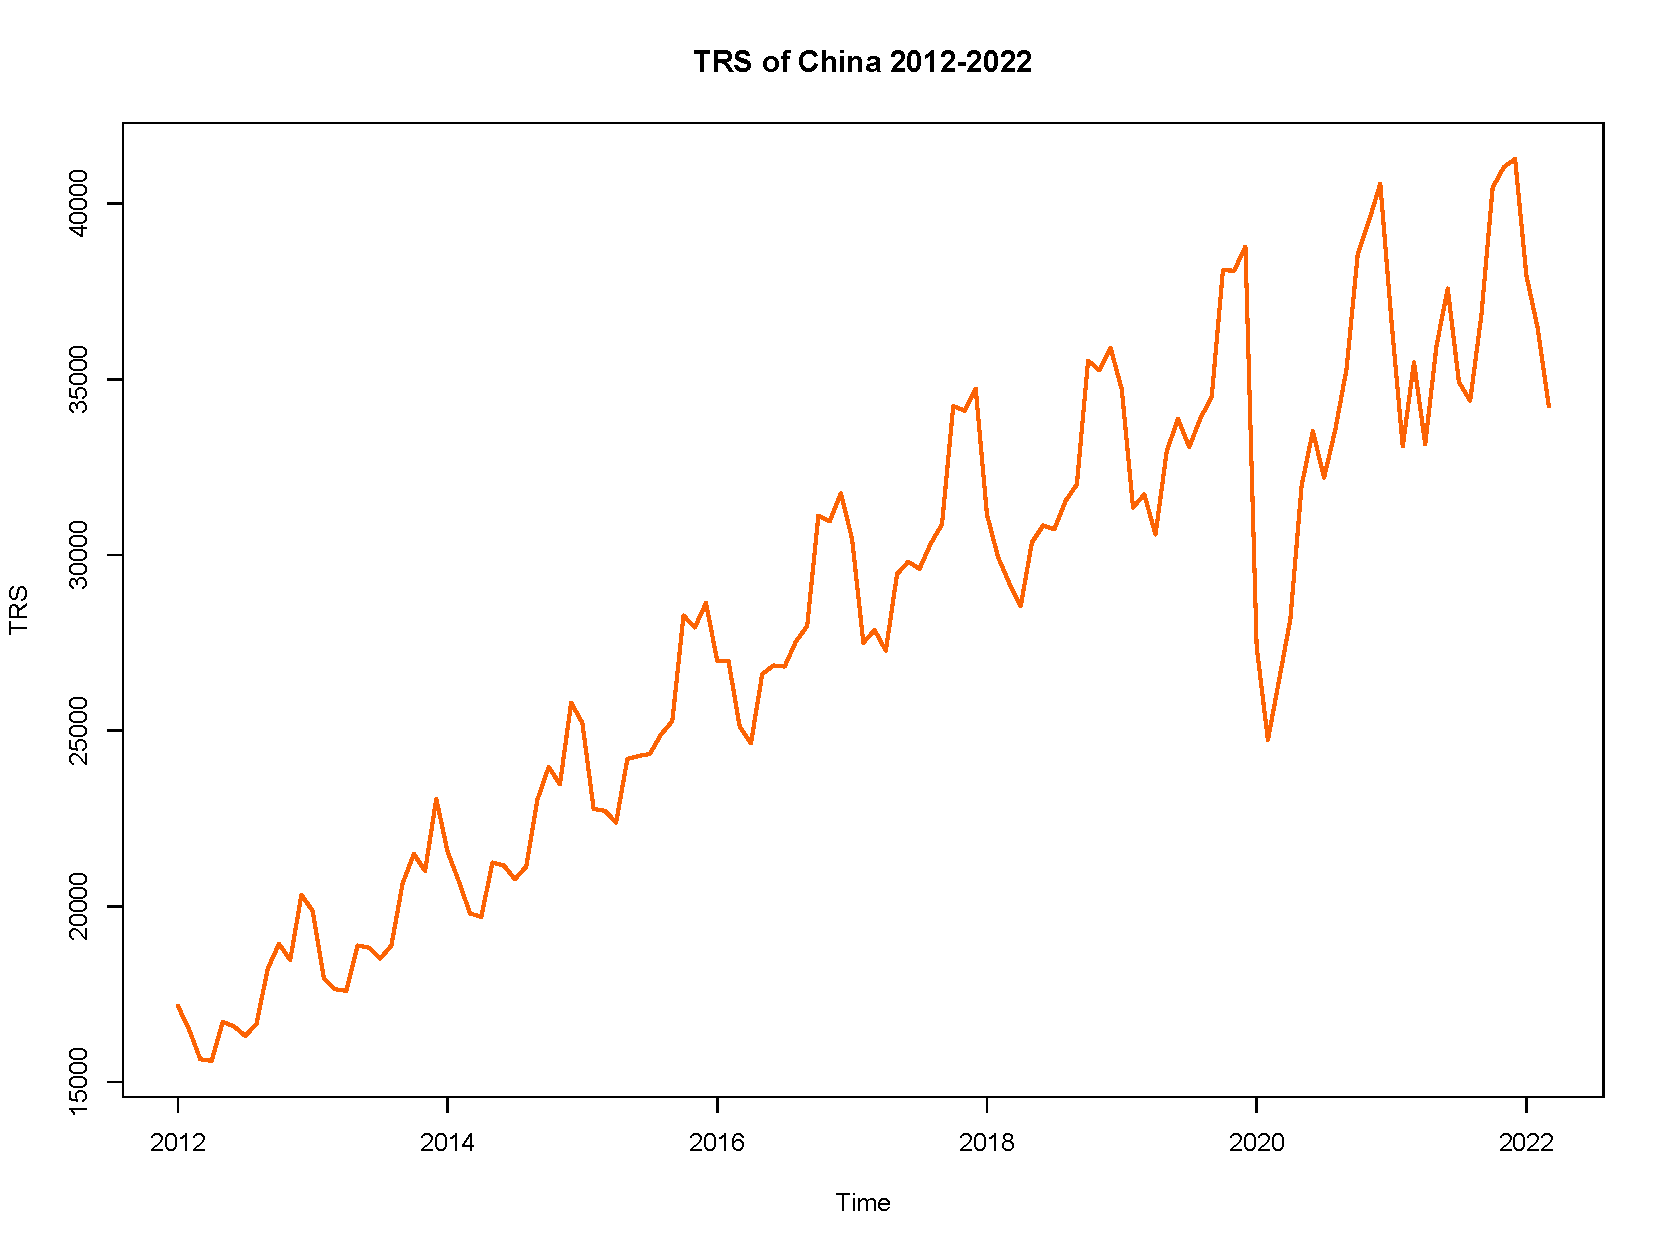
\includegraphics[width=0.6\textwidth]{Raw_TRS.pdf} %插入图片,[]中设置图片大小,{}中是图片文件名
  \caption{社会消费品零售总额2012-2022} %最终文档中希望显示的图片标题
  \label{TRS} %用于文内引用的标签
  \end{figure} 
\subsection{季节性分解}
可以看出社会消费品零售总额的变化呈明显的季节波动,并且呈现逐年上升趋势,
所以考虑通过STL算法用Loess平滑化后将时间序列数据分解为
趋势因子(trend compoents),季节因子(season compoents),和随机误差因子(remmainder compoents)\cite{stl}:
\begin{equation}
  Y_t = T_t + S_t + R_t
\end{equation}

得到分解图如下:
\begin{figure}[htbp] %H为当前位置,!htb为忽略美学标准,htbp为浮动图形
  \centering %图片居中
  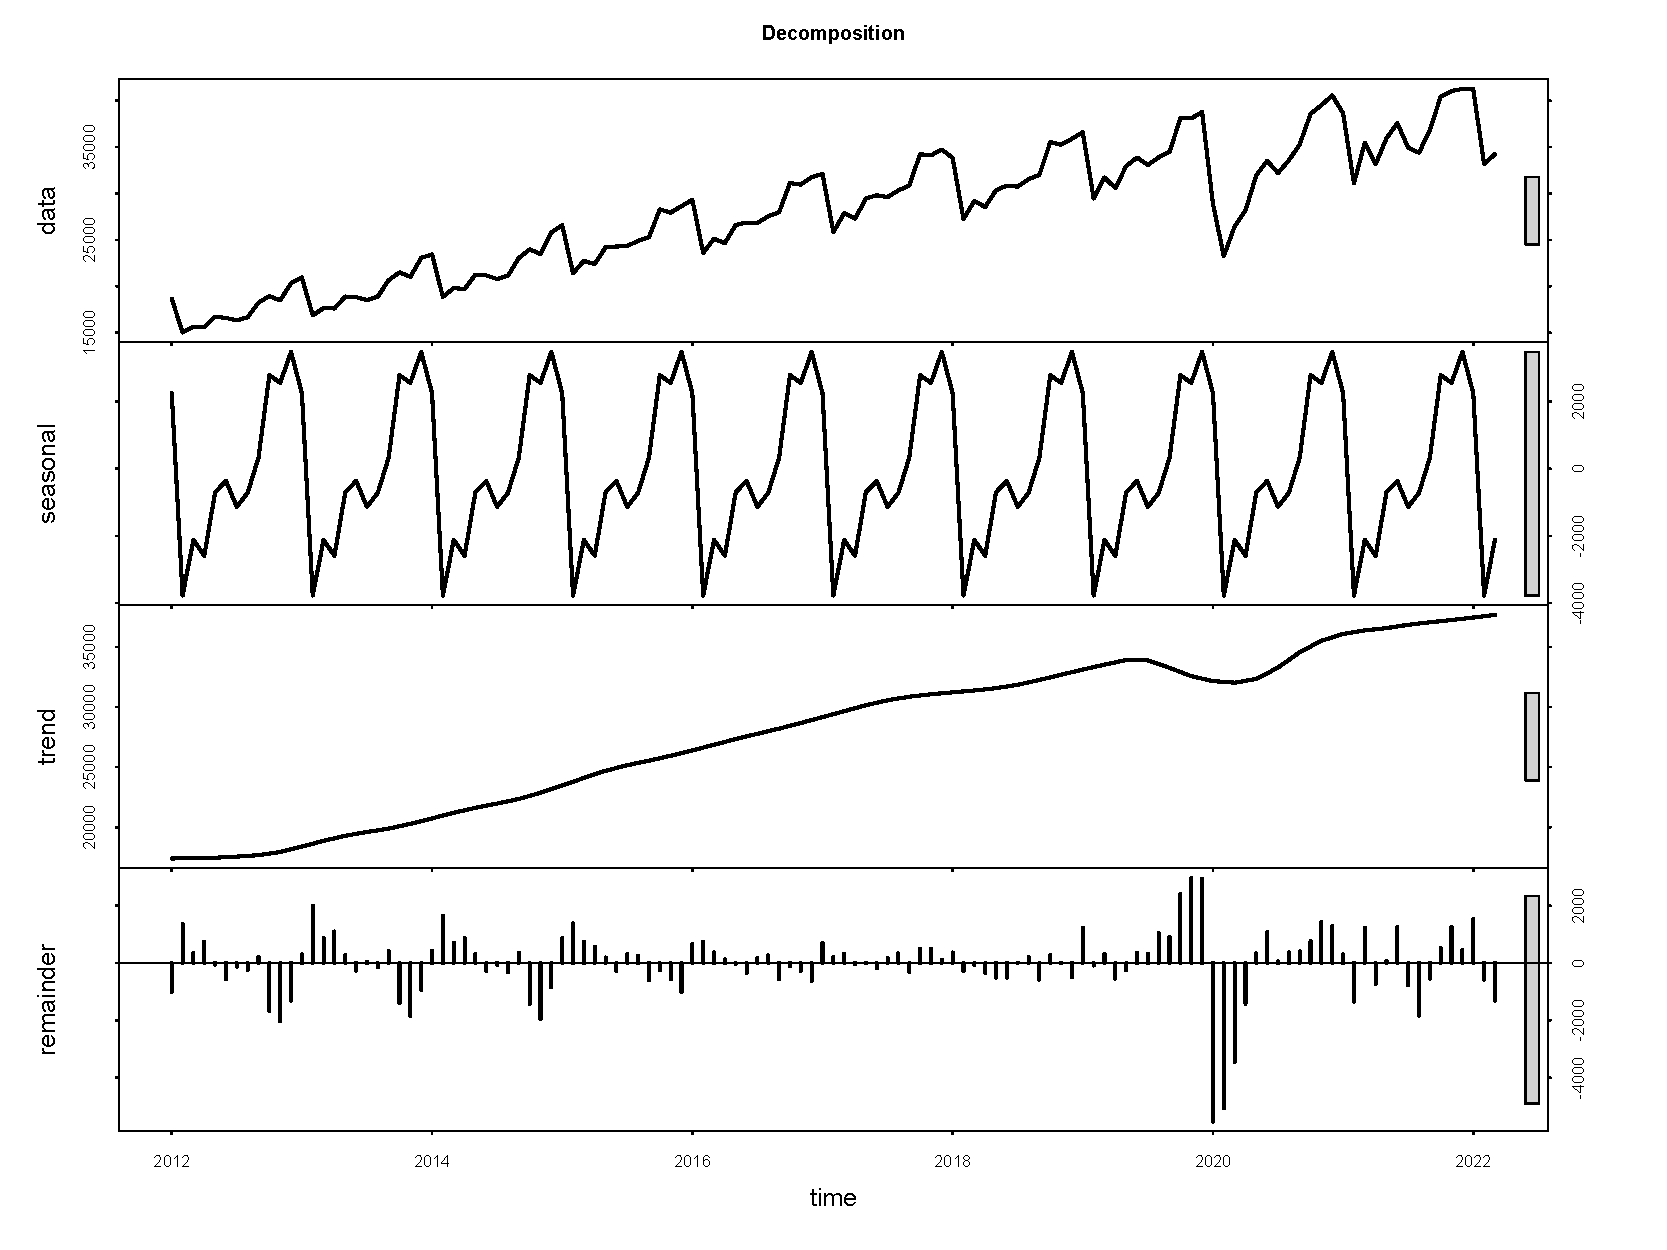
\includegraphics[width=1\textwidth]{decompose.pdf} %插入图片,[]中设置图片大小,{}中是图片文件名
  \caption{按加法模型分解后} %最终文档中希望显示的图片标题
  \label{decompose} %用于文内引用的标签
\end{figure} 

从趋势因子来看,总体趋势稳步提升直至2020疫情爆发前,到2020年末基本恢复
正常发展水平,持续稳步发展到2022年2月。
 \par 从季节因子来看,在春节前,即年末12月份,消费达到顶峰,之后逐步下降至四月份到达最低点,之后开始逐步攀升
直至12月份。
\section{数据检验}

\subsection{时序平稳性检验}
若时间序列\(X_t\)满足如下条件:

  (1) 均值\(E ( X_t ) = \mu \),均值\(\mu\)是与时间\(t\)无关的常数

  (2) 方差\(Var(X_t) = \sigma^2\),方差\(\sigma\)是与时间\(t\)无关的常数

  (3) 协方差\(Cov(X_t,X_t+k) = \gamma^2\),协方差只与间隔\(t\)有关  

  则称时间序列\(X_t\)是平稳的。

由表\ref{TRS}中可明显看出均值随时间\(t\)增长,可以猜测原序列应为非平稳序列。
采用\(ADF\)检验原序列的平稳性,\(ADF\) 检验通过一下三个模型检验:
\begin{equation}
  \begin{aligned}
  &\Delta X_t = \delta X_{t-1} + \sum_{i=1}^{m}\beta_i X_{t-i} + \epsilon_t \\
  &\Delta X_t =\alpha + \delta X_{t-1} + \sum_{i=1}^{m}\beta_i X_{t-i} + \epsilon_t \\
  &\Delta X_t =\alpha +\beta_t+ \delta X_{t-1} + \sum_{i=1}^{m}\beta_i X_{t-i} + \epsilon_t
  \end{aligned}
\end{equation}

三个模型原假设都是\(H_0 : \delta = 0\) 若拒绝\(H_0\)则为平稳序列,否则为非平稳序列。
通过\(ADF \)临界值表判断是否接受\(H_0\)

为验证猜想对原序列做\(ADF\)检验,得到结果如下:
% Table generated by Excel2LaTeX from sheet 'Sheet1'
\begin{table}[htb]
  \centering
  \caption{Add caption}
    \begin{tabular}{lr}
    \multicolumn{2}{c}{ Augmented Dickey-Fuller Test} \\
    \hline
    Lag Order: & 1 \\
    Dickey-Fuller: & 0.3394\\
    P Value  & 0.7218 \\
    \end{tabular}%
  \label{tab:ADF_raw}%
\end{table}%

由于\(p-value > 0.05 \)所以无法拒绝原假设,因此原序列是非平稳的。
为了将原序列转化为平稳序列处理,因为从图\ref{TRS}看出原序列应该
有随时间线性增加的趋势,考虑对原序列做一阶差分\cite{Rob},得到新序列\(\hat{X}_t\)如下图:
\begin{figure}[H] %H为当前位置,!htb为忽略美学标准,htbp为浮动图形
  \centering %图片居中
  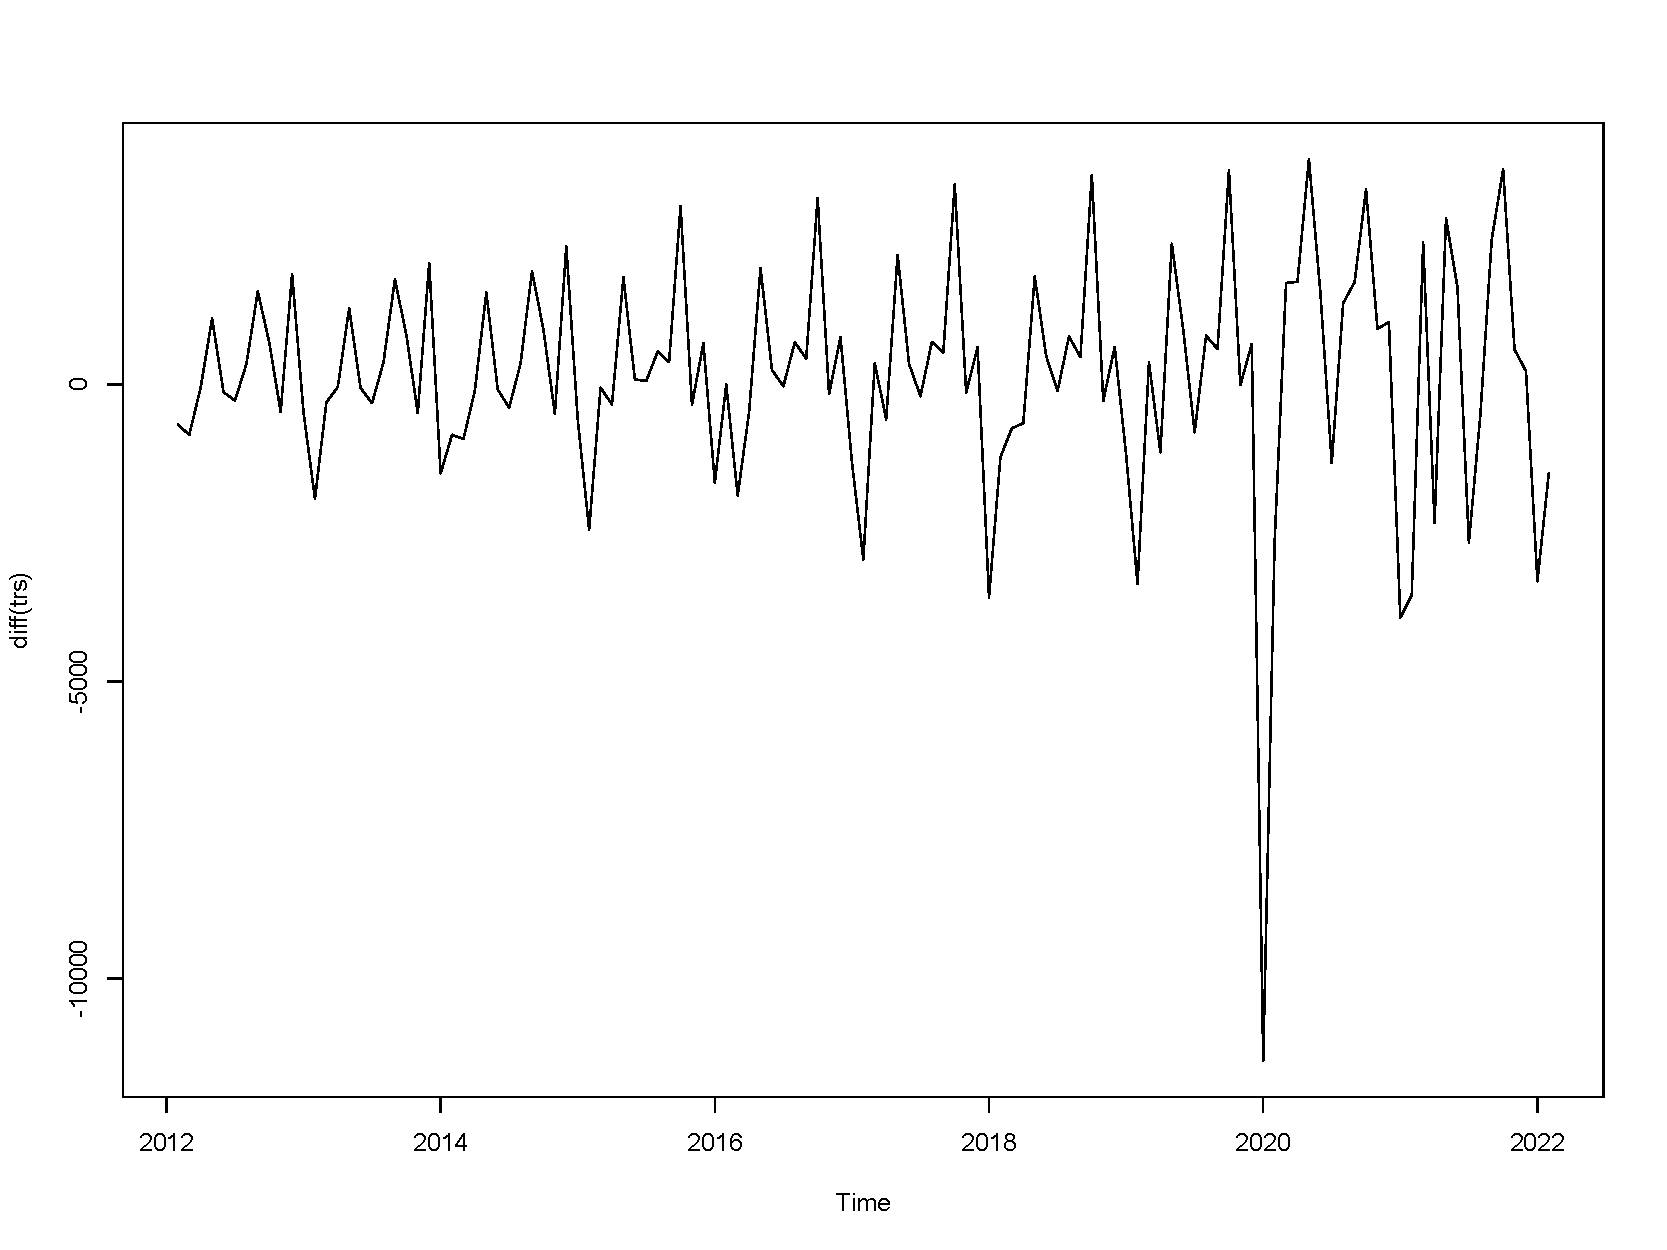
\includegraphics[width=0.7\textwidth]{diff_TRS.pdf} %插入图片,[]中设置图片大小,{}中是图片文件名
  \caption{对原序列做一阶差分后} %最终文档中希望显示的图片标题
  \label{diff_TRS} %用于文内引用的标签
\end{figure} 

在对差分后的序列做\(ADF\)检验:
\begin{table}[H]
  \centering
  \caption{\(ADF\)检验}
    \begin{tabular}{lr}
    \multicolumn{2}{c}{ Augmented Dickey-Fuller Test} \\
    \hline
    Lag Order: & 1 \\
    Dickey-Fuller: & -7.5267\\
    P Value  & 0.01 \\
    \end{tabular}%
  \label{tab:ADF_diff}%
\end{table}%

由于\(p<0.05\)所以拒绝原假设,差分后的序列是平稳的,
即通过一阶差分去掉了原序列线性的趋势因子。

\subsection{数据随机性检验}
尽管\(\hat{x}_t\)为平稳序列,但是如白噪声等纯随机序列
也是平稳序列,若\(\hat{X}_t\)是纯随机序列,则没有建模研究价值
价值,于是采用\(Ljung-Box\)检验随机性

假设\(H_0:\rho _1 = \rho _2 = \cdots = \rho _n = 0\)
则对所有的\(k>0\),样本的自相关系数服从:
\begin{equation}
  \hat{\rho}_k \approx N(0,\frac{1}{n})
\end{equation}

其中\(n\)为样本量,通过检验统计量:
\begin{equation}
  Q_{LB}(m) = n (n+2)\sum_{k=1}^{m}{\frac{\hat{\rho_{k}}^2}{n-k}} ~\chi^2(m)
\end{equation}

得到的\(Ljung-Box\)检验结果为:
% Table generated by Excel2LaTeX from sheet 'Sheet1'
\begin{table}[H]
  \centering
  \caption{\(Ljung-Box\)检验}
    \begin{tabular}{ll}
    \multicolumn{2}{c}{Ljung-Box test} \\
    \hline
    X-squared  & \multicolumn{1}{r}{494.39} \\
    df    & \multicolumn{1}{r}{6} \\
    p-value & < 2.2e-16 \\
    \end{tabular}%
  \label{tab:Ljung-Box}%H
\end{table}%

由于\(p<0.05\)所以拒绝原假设,则\(\hat{X}_t\)为非随机序列,可进行下一步建模。



\section{模型建立}
\subsection{无季节性的ARIMA模型建立}
给定一个差分\(d\)阶的时间序列\(y_t\),\(ARIMA(p,d,q)\)模型如下:
\begin{equation}
  y_t'=c+\sum_{i=1}^p{\phi_i y_{t-i}}+\sum_{i=1}^q{\theta_i\varepsilon_{t-i}}+\varepsilon_t
\end{equation}

其中\(\varepsilon_t\)是白噪声序列, \(p\)是自回归的阶数,\(q\)是移动平均的阶数。

平稳序列的自相关函数\(ACF\)与时间间隔\(k\)有关,并通过\(ACF\)相关系数决定\(q\):
\begin{equation}
  \rho_h = \rho(y_t,y_{t+k}) =\frac{Cov(y_t,y_{t+k})}{\sigma_t \sigma_{t+k}}
\end{equation}

\(ACF\)图显示了\(y_t\)与\(y_{t-k}\)之间相关性,但是滞后阶数\(1,2,\cdots,k-1\)之间存在依赖
关系,例如若\(y_t\)与\(y_{t-1}\)自相关,那么\(y_t\)与\(y_{t-2}\)一定自相关,
因为他们都通过与\(y_{t-1}\)直接相关,而间接自相关,为了分离\(y_{t-1},
y_{t-2},\cdots,y_{t-k+1}\)的干扰,直接得到\(y_t\)与\(y_{t-k}\)之间的相关性,
\(y_{t-k}\)之间的向通过\(PACF\)估计\(P\)值,由于历史白噪声\(\varepsilon_{t-k}\)通过影响历史观测值来间接影响
当前\(y_t\)所以用\(ACF\)估计\(q\)值,绘出一阶差分后\(\hat{X}_t\)的\(ACF\)和\(PACF\)图(临界值\(\frac{\pm1.96}{T}\)以用虚线标出):
\begin{figure}[H] %H为当前位置,!htb为忽略美学标准,htbp为浮动图形
  \centering %图片居中
  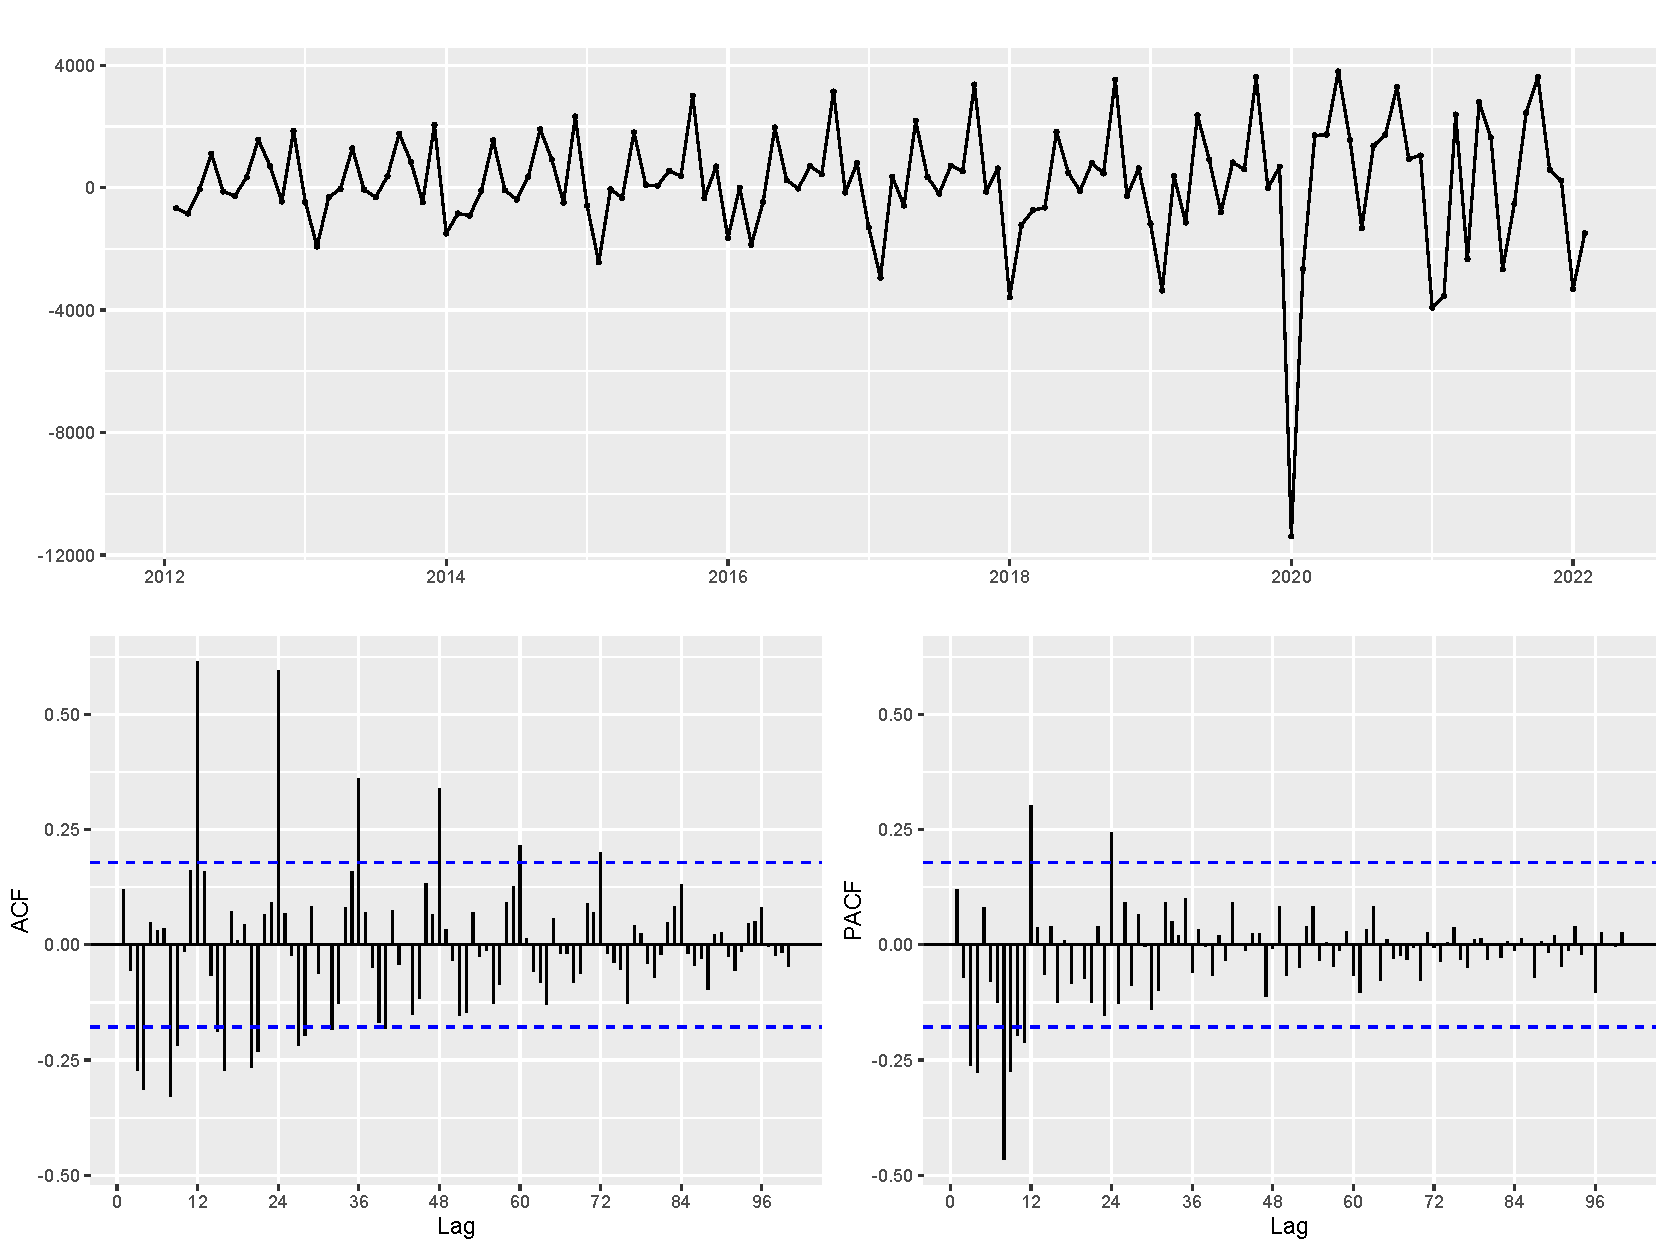
\includegraphics[width=1\textwidth]{acf_pacf.pdf} %插入图片,[]中设置图片大小,{}中是图片文件名
  \caption{ACF 和 PACF} %最终文档中希望显示的图片标题
  \label{acf_pacf} %用于文内引用的标签
  \end{figure} 
  \subsection{季节性的ARIMA模型}
  通过图\ref{acf_pacf}发现在滞后阶数\(lag\)值很高时才出现拖尾,会导致参数过多发生
  过拟合现象, 而且通过图\ref{decompose}得到消费总额应该是呈现明显季节波动
  所以考虑将一阶差分序列\(\hat{X}_t\)分解为季节部分和剩下的非季节部分:
\begin{center}
  ARIMA\;\;\;\;	\((p, d, q)\)	\;\;\;\;\; \((P, D, Q)_{m}\) \label{Season_decompose}
\end{center}

其中\(m=12\)为观测周期,可以将模型写成季节
部分与非季节部分的乘积,例如对于\(ARIMA(1,1,1)(1,1,1)_m\)
模型:
\begin{equation}
  (1 - \phi_{1}B)~(1 - \Phi_{1}B^{12})~(1 - B)~(1 - B^{4})y_{t} = (1 + \theta_{1}B)~ (1 + \Theta_{1}B^{4})\varepsilon_{t}
\end{equation}

 \subsection{参数估计}
 为先消除季节型波动,对一阶差分后\(\hat{X}_t\)做季节性差分,得到
 \(X'_{t}\) = \(\hat{X}_t-\hat{X}_{t-12)}\),绘出相关图像:
 \begin{figure}[H] %H为当前位置,!htb为忽略美学标准,htbp为浮动图形
  \centering %图片居中
  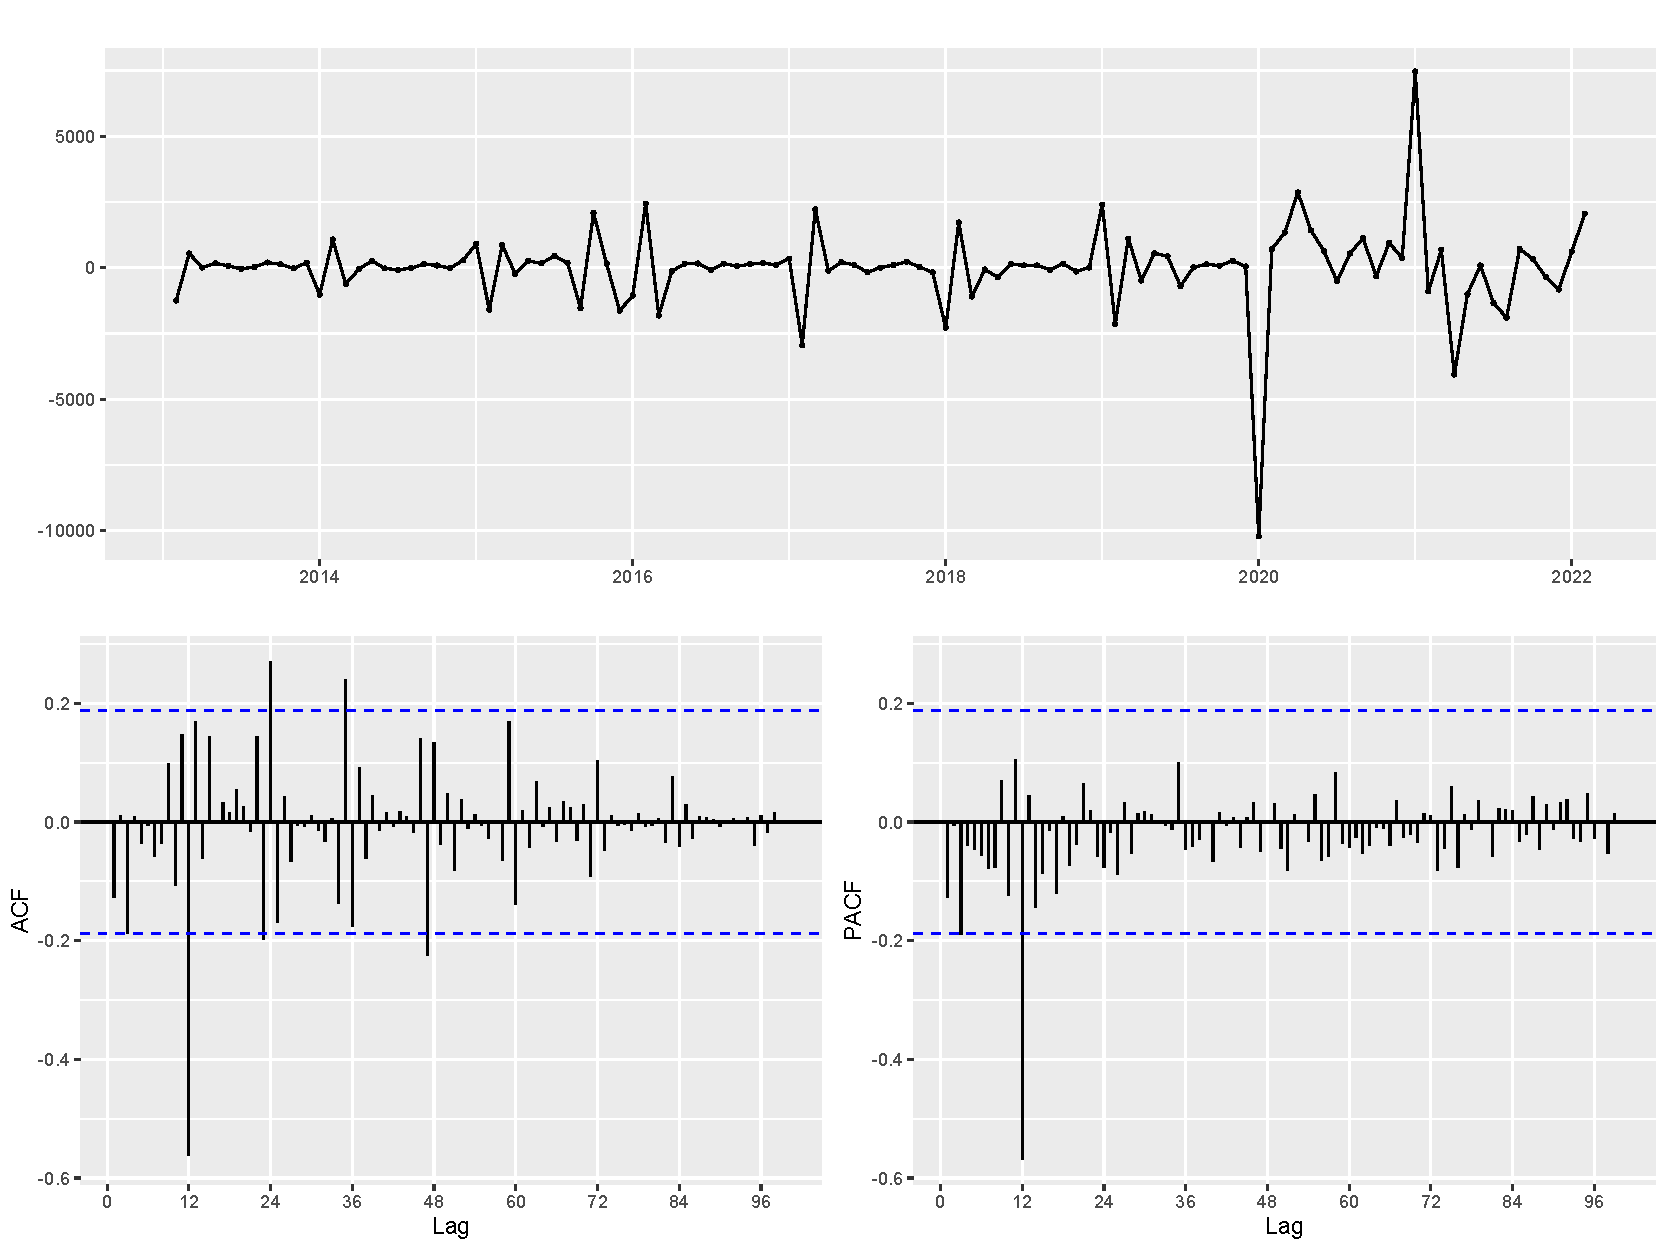
\includegraphics[width=1\textwidth]{Season_diff.pdf} %插入图片,[]中设置图片大小,{}中是图片文件名
  \caption{季节差分后 ACF 和 PACF} %最终文档中希望显示的图片标题
  \label{season_diff} %用于文内引用的标签
  \end{figure}
  \subsection*{模型的选择}
  从相关系数图看出相比于图\ref{acf_pacf}, 相关系数的的衰减速度
  加快很多,对于季节部分的ACF和PACF图(即\(Lag=12n\),二者都认为在滞后系数\(Lag=12\)后产生拖尾。
  可确定\ref{Season_decompose}中的相应系数\(P=1 , Q=1\)

  但对于非季节部分的ACF和PACF图较难判断在何种滞后系数后产生拖尾,因此利用AIC,AICc,BIC准则定量的确定在何种
  系数下的模型最优:
  \begin{equation*}
    \text{AIC} = -2log(L) + 2(p+q+k+1)
  \end{equation*}
  其中\(L\)是似然数据的似然函数,最后一项为参数个数(包含了余项的方差)\(k=0\)若\(c=0\),\(k=1\)若\(c\neq0\)
  对于ARIMA模型而言,修正过的AIC值可以被表示为:
  \begin{equation*}
    \text{AICc} = \text{AIC} + \frac{2(p+q+k+1)(p+q+k+2)}{T-p-q-k-2}
  \end{equation*}

  并且贝叶斯信息准则(BIC)如下:\[\text{BIC} = \text{AIC} + [\log(T)-2](p+q+k+1)\]
  通过枚举p,q的值得到相应模型AIC,AICc,BIC如下:
  % Table generated by Excel2LaTeX from sheet 'Sheet1'
\begin{table}[H]
  \centering
  \caption{不同系数对应检测值}
    \begin{tabular}{cccc}
    相应的ARIMA模型 & AIC   & AICc  & BIC \\
    \hline
    (0,1,0)(1,1,1)[12] & 1858.76 & 1858.99 & 1866.81 \\
    (0,1,1)(1,1,1)[12] & 1860.45 & 1860.84 & 1871.18 \\
    (0,1,2)(1,1,1)[12] & 1859.87 & 1860.46 & 1873.28 \\
    (0,1,3)(1,1,1)[12] & 1857.89 & 1858.72 & 1873.98 \\
    (1,1,0)(1,1,1)[12] & 1860.53 & 1860.92 & 1871.26 \\
    (1,1,1)(1,1,1)[12] & 1853.79 & 1854.38 & 1867.2 \\
    (1,1,2)(1,1,1)[12] & 1855.14 & 1855.98 & 1871.24 \\
    (1,1,3)(1,1,1)[12] & 1857.04 & 1858.16 & 1875.81 \\
    (1,1,4)(1,1,1)[12] & 1859.01 & 1861.57 & 1883.87 \\
    (2,1,1)(1,1,1)[12] & 1855.09 & 1855.92 & 1871.19 \\
    (2,1,2)(1,1,1)[12] & 1856.44 & 1857.56 & 1875.21 \\
    (2,1,3)(1,1,1)[12] & 1858.1 & 1858.18 & 1875.83 \\
    (3,1,1)(1,1,1)[12] & 1857.06 & 1858.18 & 1875.83 \\
    \end{tabular}%
  \label{choose optimal models}%
\end{table}%
  从表\ref{choose optimal models}中看出,\(ARIMA(1,1,1)(1,1,1)_{12}\)是最优的ARIMA模型。
  \subsection{残差检验}
  为说明残差纯随机变量,对残差做Ljung-Box test检验:
  \begin{table}[H]
    \centering
    \caption{残差\(Ljung-Box\)检验结果}
      \begin{tabular}{ll}
      \multicolumn{2}{c}{Ljung-Box test} \\
      \hline
      df    & \multicolumn{1}{r}{20} \\
      p-value & 0.97 \\
      \end{tabular}%
    \label{Ljung-Box of Residuals}%H
  \end{table}%
  \(p>0.05\)无法拒绝原假设,所得残差为白噪声序列,残差之间不存在自相关性。
  并且得到的残差图\ref{Redsiduals},残差基本符合正态分布要求:
  \begin{figure}[H] %H为当前位置,!htb为忽略美学标准,htbp为浮动图形
  \centering %图片居中
  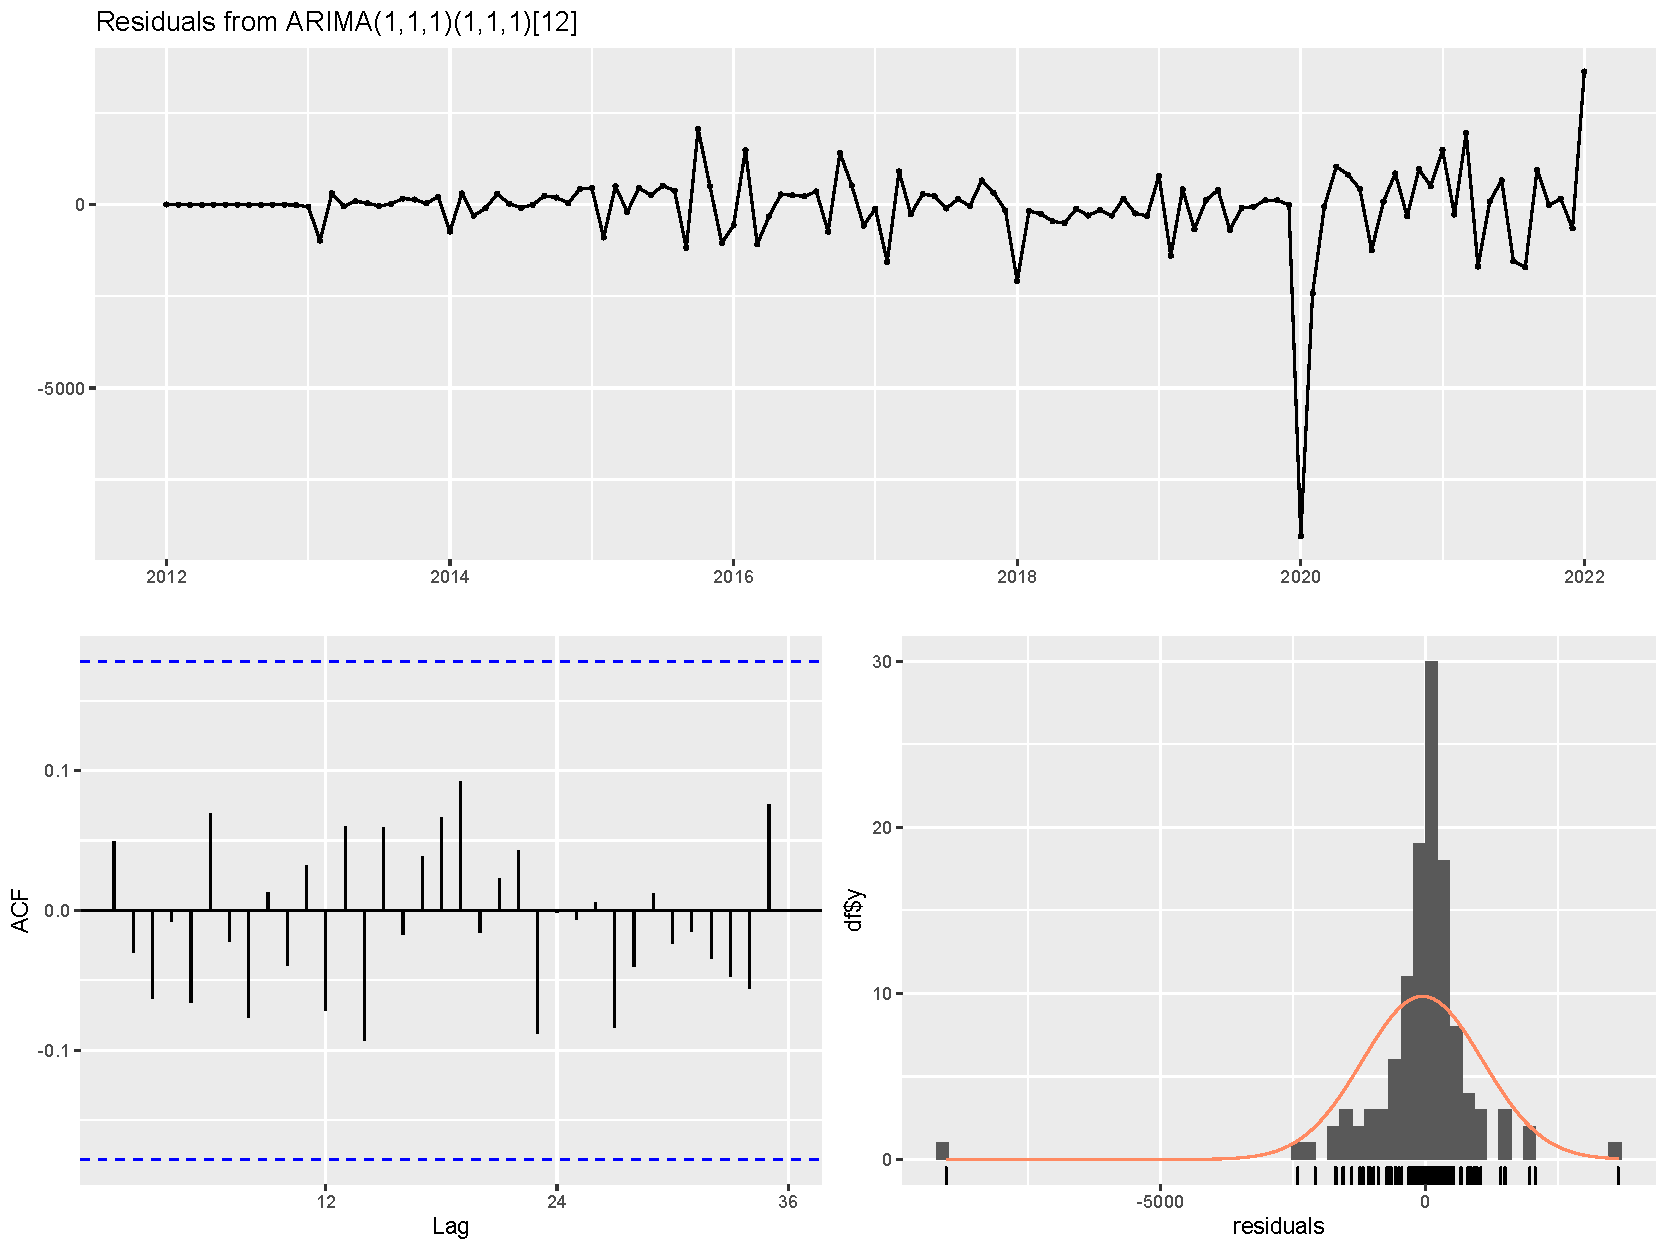
\includegraphics[width=0.8\textwidth]{Residuals.pdf} %插入图片,[]中设置图片大小,{}中是图片文件名
  \caption{\(ARIMA(1,1,1)(1,1,1)_{12}\)的残差图} %最终文档中希望显示的图片标题
  \label{Redsiduals} %用于文内引用的标签
  \end{figure} 
  为进一步说明,绘出正态Q-Q图\ref{Q-Qplot},所以残差符合正态分布要求:
  \begin{figure}[H] %H为当前位置,!htb为忽略美学标准,htbp为浮动图形
    \centering %图片居中
    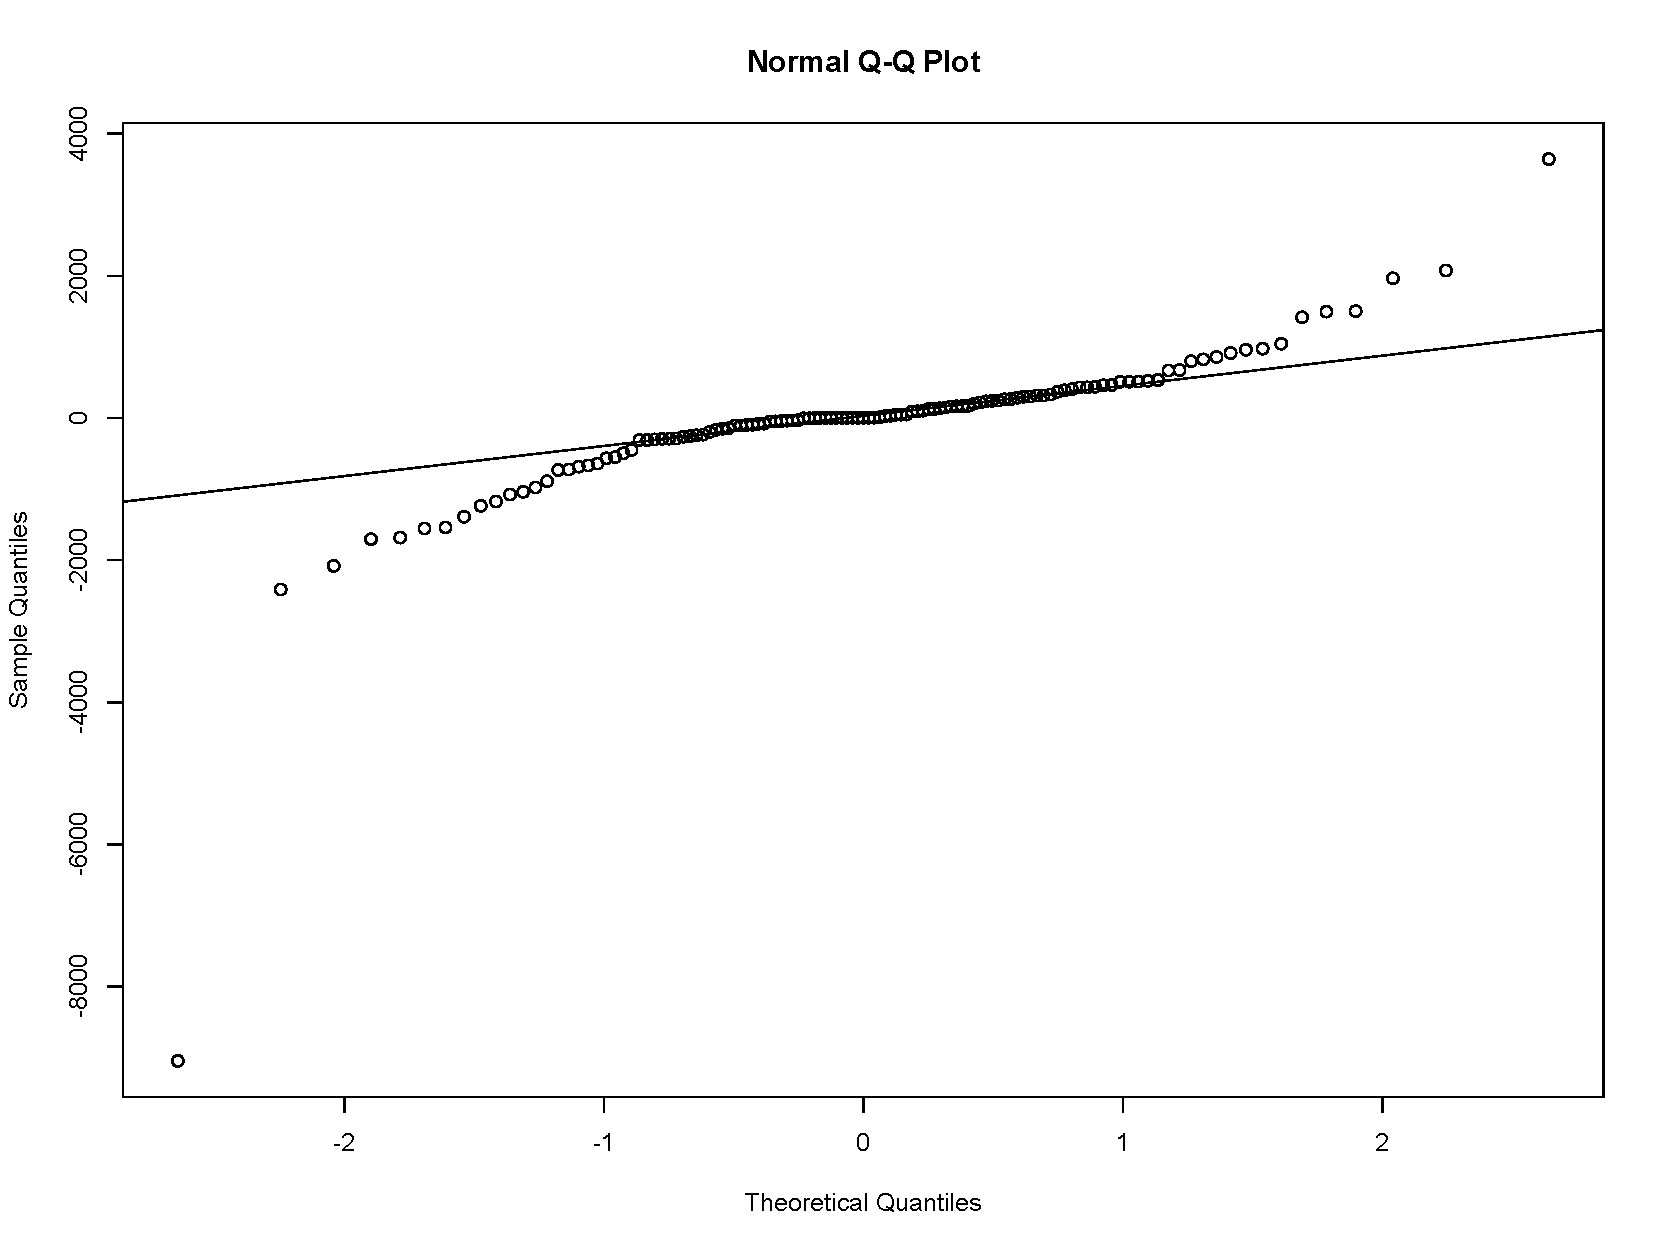
\includegraphics[width=0.8\textwidth]{Q-Qplot.pdf} %插入图片,[]中设置图片大小,{}中是图片文件名
    \caption{\(ARIMA(1,1,1)(1,1,1)_{12}\)的残差Q-Q图} %最终文档中希望显示的图片标题
    \label{Q-Qplot} %用于文内引用的标签
  \end{figure} 
  \subsection{预测}
  选取的训练集为表\ref{TRS}中2022年2月以前(包括二月).
  用得到的ARIMA模型对训练集进行拟合,以12个月划分序列。
  通过所有之前的数据拟合当前年份的数据(起始两年除外),拟合得到的12步拟合结果图\ref{traning_forecast}:
  \begin{figure}[H] %H为当前位置,!htb为忽略美学标准,htbp为浮动图形
    \centering %图片居中
    \begin{minipage}[t]{0.48\textwidth}
      \centering
      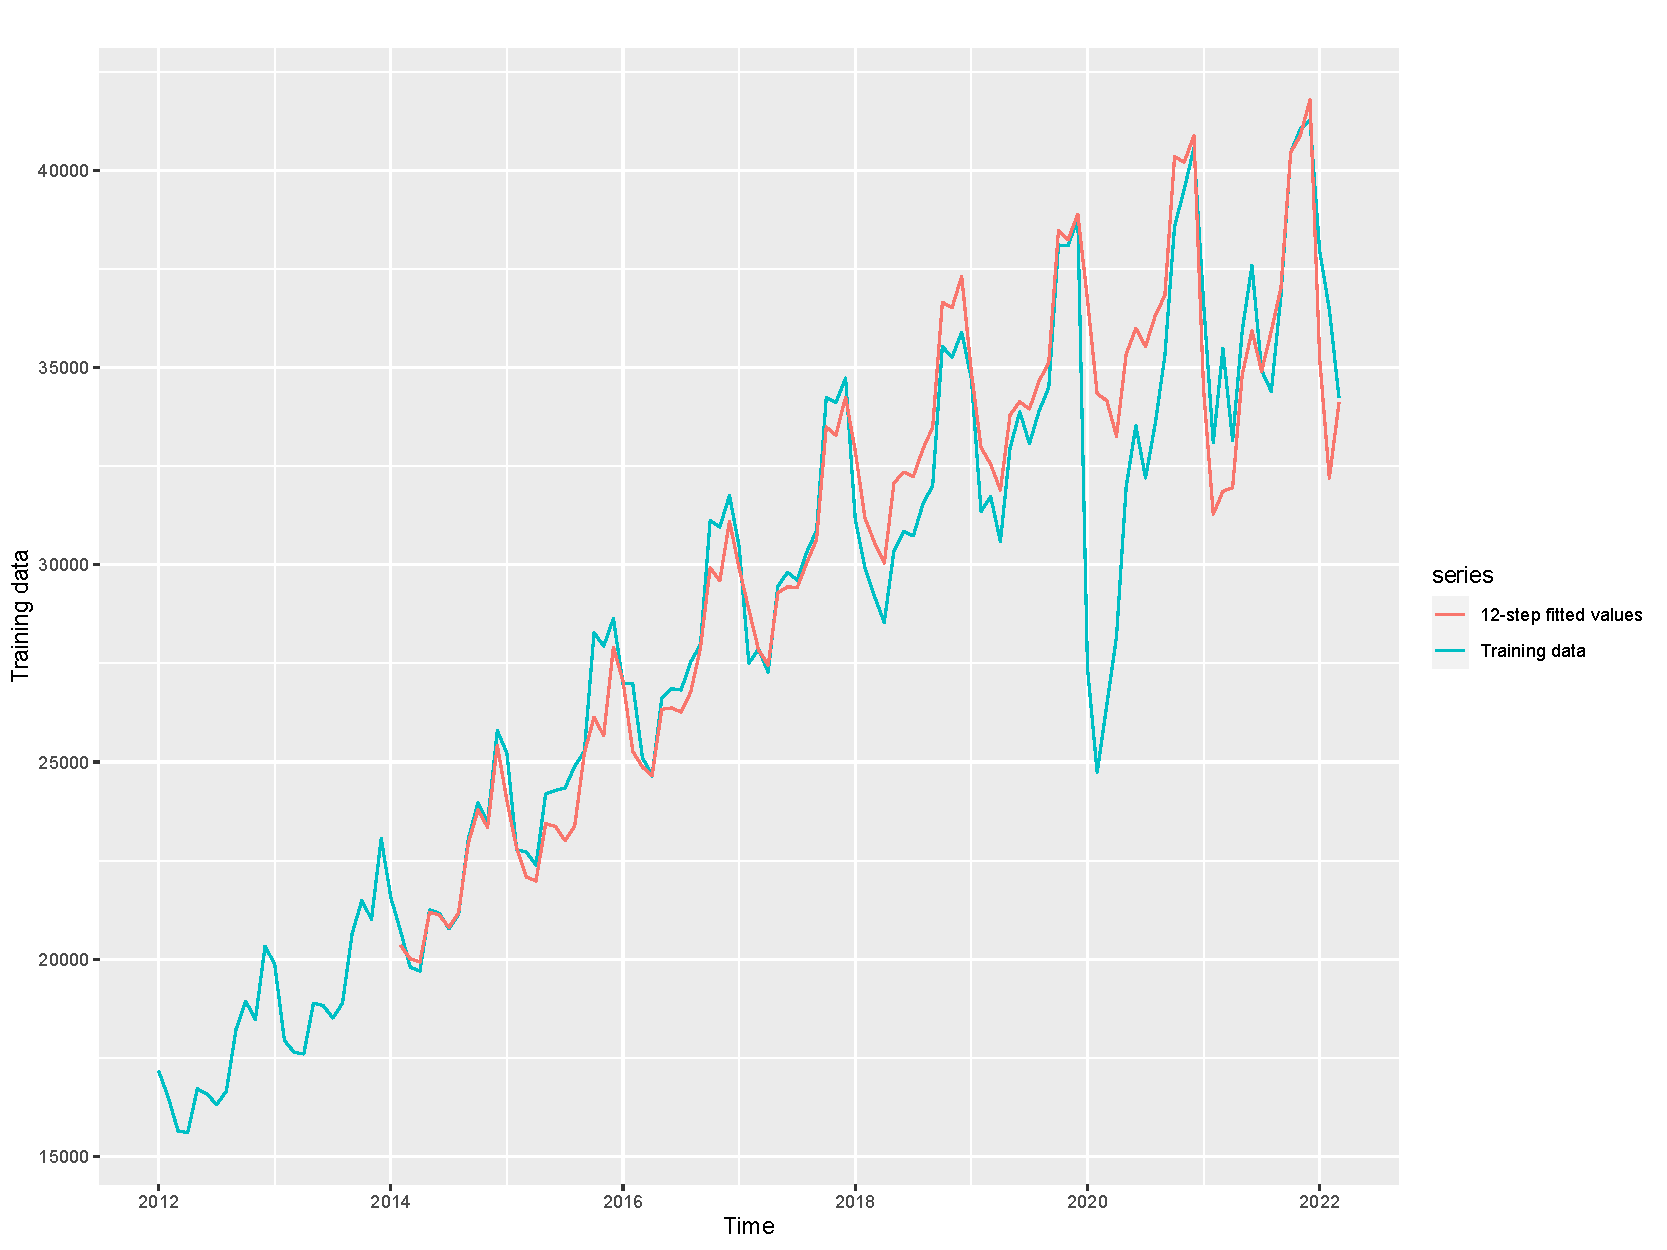
\includegraphics[width=1\textwidth]{training_forecast.pdf} %插入图片,[]中设置图片大小,{}中是图片文件名
      \caption{\small{\(ARIMA\)模型得到的12步拟合值}} %最终文档中希望显示的图片标题
      \label{traning_forecast} %用于文内引用的标签
    \end{minipage}
    \begin{minipage}[t]{0.48\textwidth}
      \centering %图片居中
      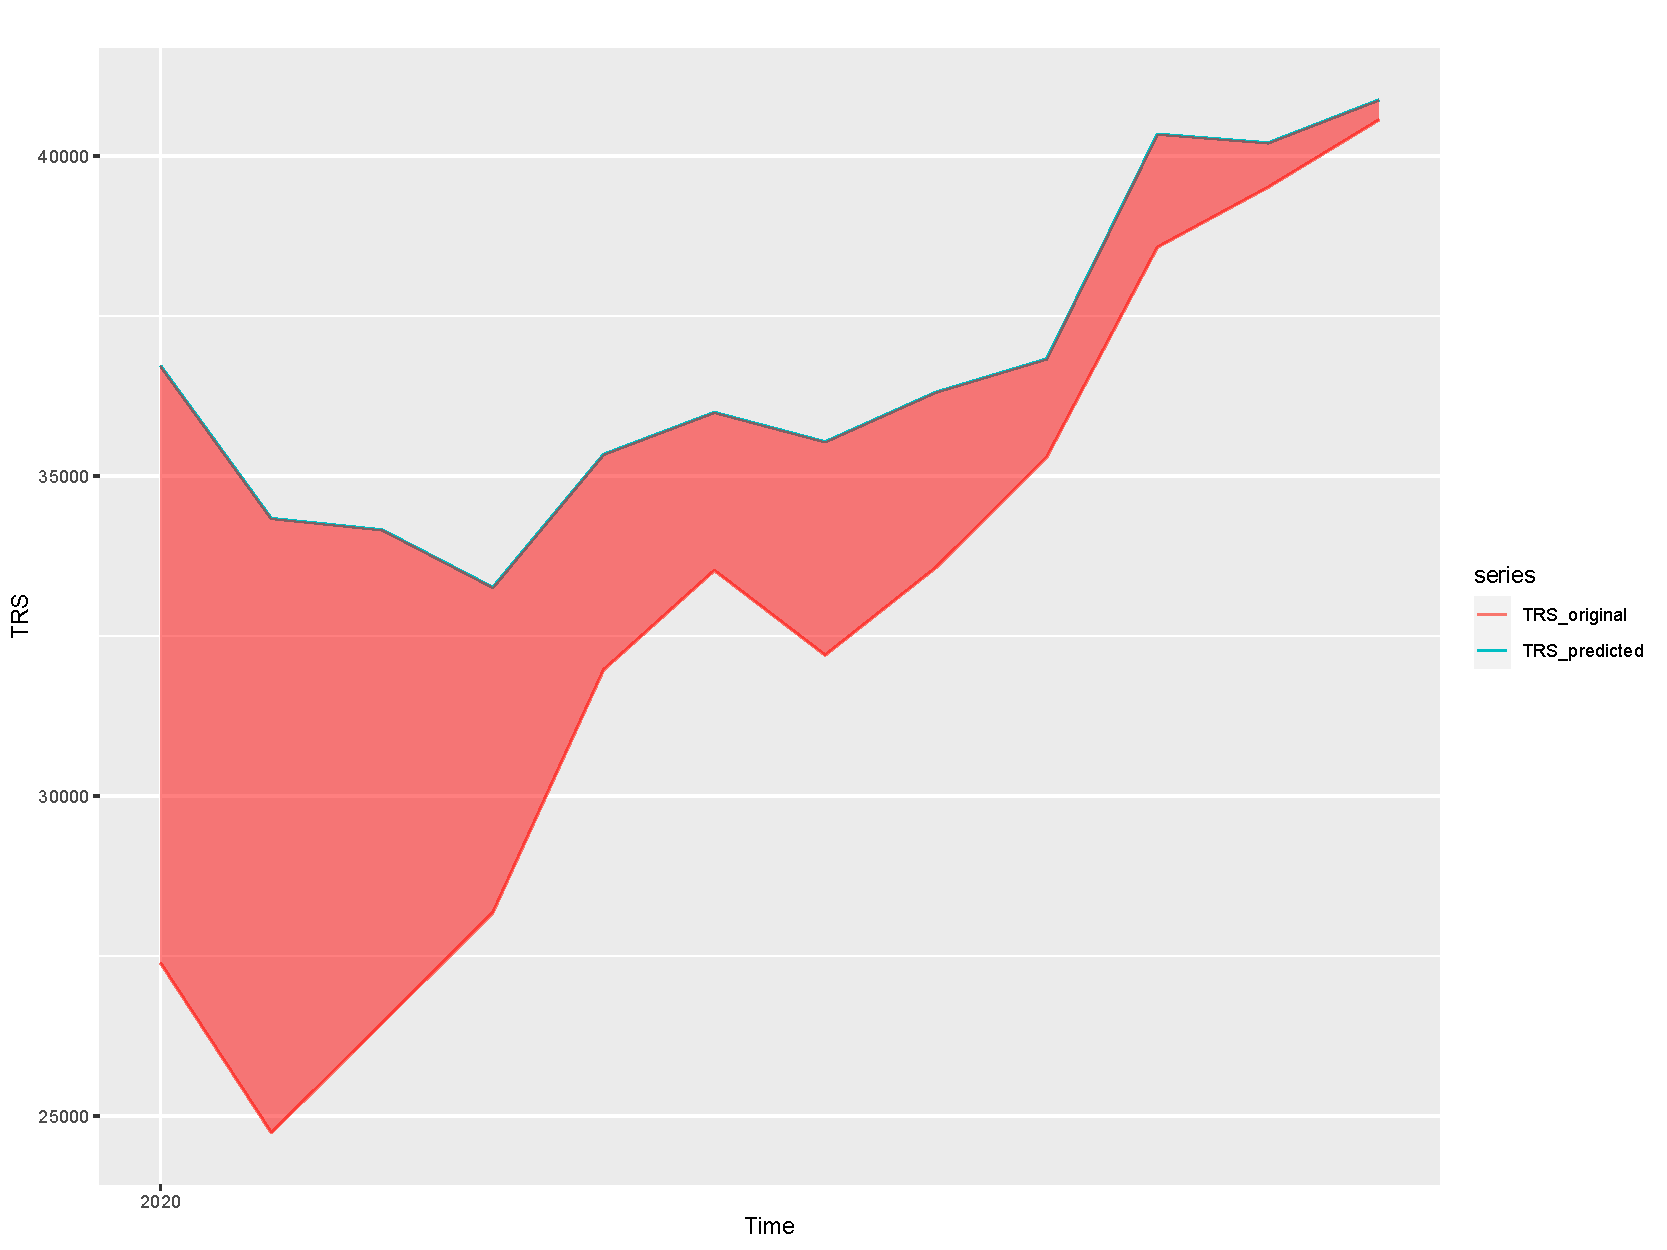
\includegraphics[width=1\textwidth]{trs_2020.pdf} %插入图片,[]中设置图片大小,{}中是图片文件名
      \caption{\small{2020年社会消费品零售总额的损失}} %最终文档中希望显示的图片标题
      \label{trs_2020} %用于文内引用的标签
    \end{minipage}
  \end{figure} 
  从图像上看,出去2020年初有所偏差外,其余部分都能较好拟合。由此也能从图中得出2020年
  疫情带来的社会消费品零售总额的损失为47934.05(亿元),为图\ref{trs_2020}中阴影部分。
  最终用此模型预测自2022年3月起6个月的预测结果如下,并给出\(80\% \text{和}95\%\)的置信区间。
  \begin{figure}[H] %H为当前位置,!htb为忽略美学标准,htbp为浮动图形
    \centering %图片居中
    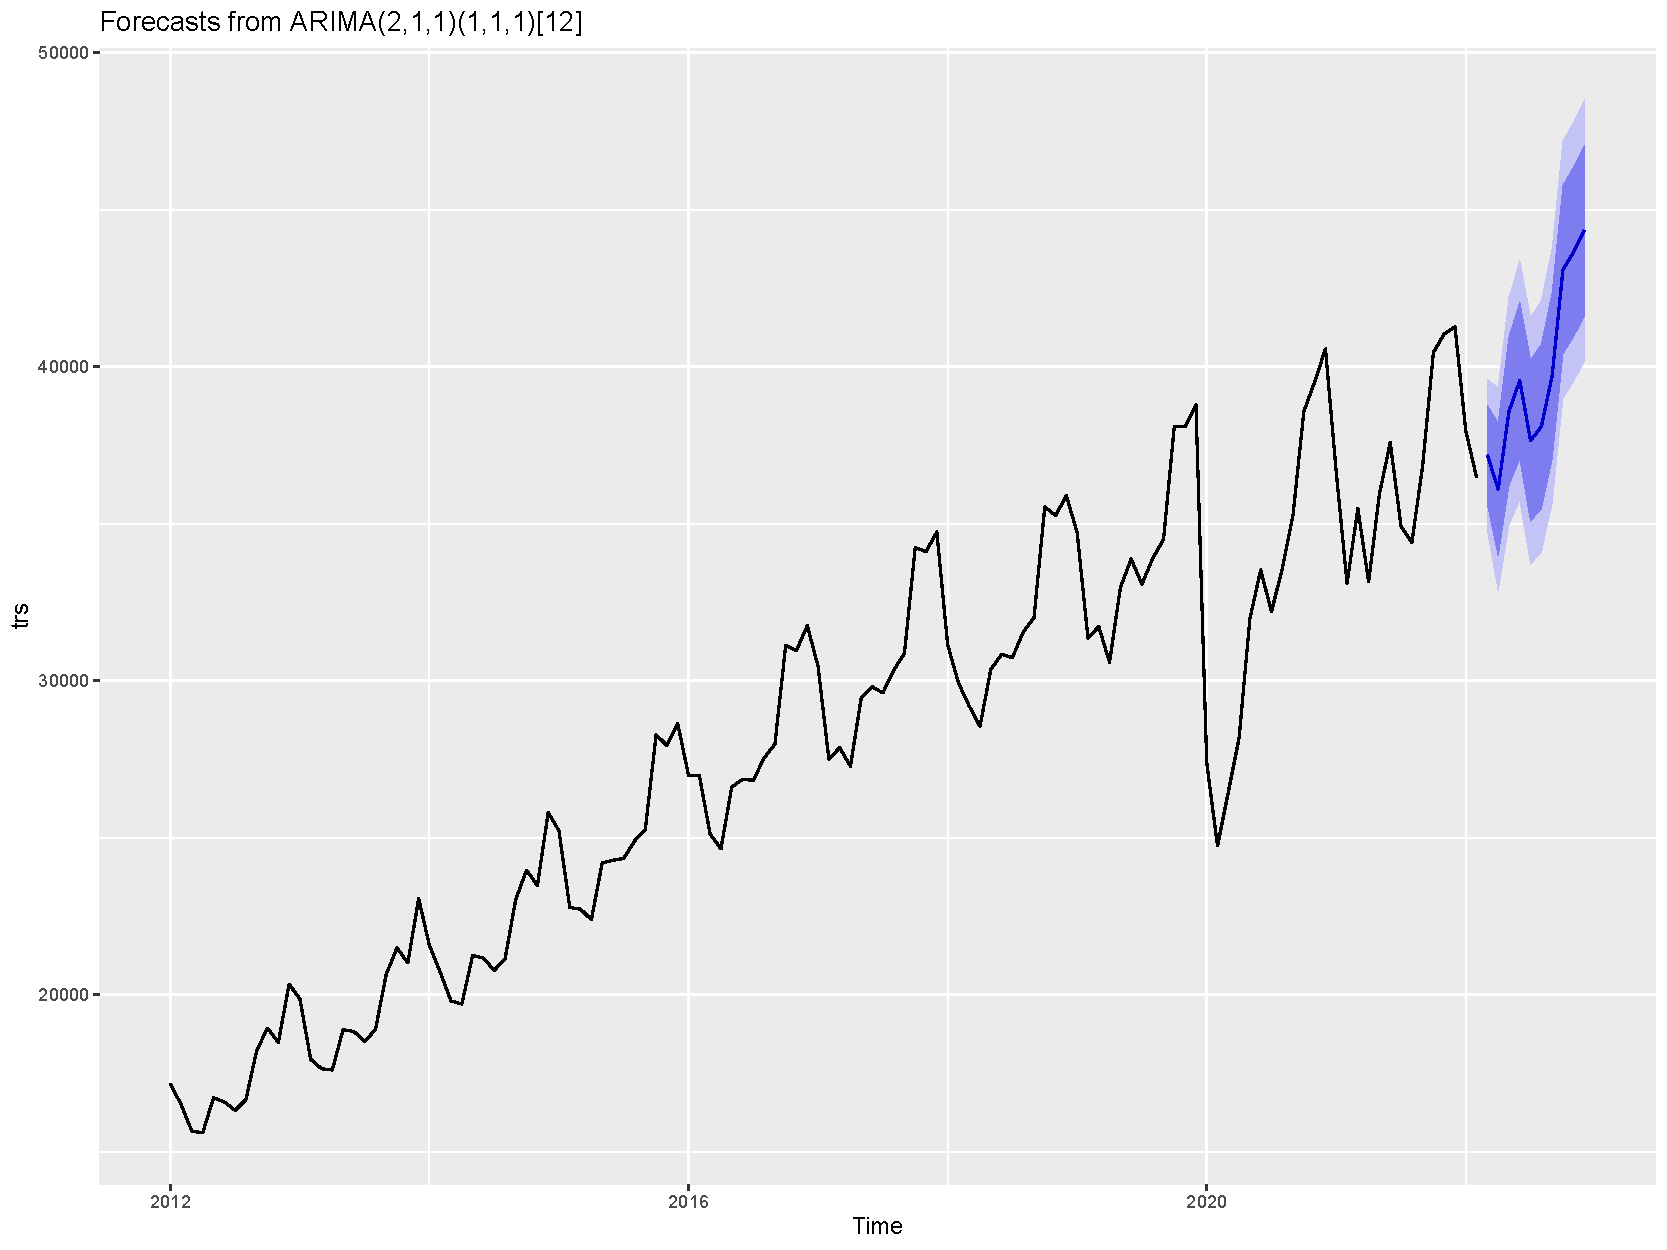
\includegraphics[width=0.7\textwidth]{forecast.pdf} %插入图片,[]中设置图片大小,{}中是图片文件名
    \caption{\(ARIMA(1,1,1)(1,1,1)_{12}\)模型对从3月起6个月的预测} %最终文档中希望显示的图片标题
    \label{forecast} %用于文内引用的标签
  \end{figure} 
  \section{干预分析模型的建立}
  \subsection{模型建立}
  假设疫情对经济的影响是突然开始,并且持续的,对持续性干预变量
  \[S_t^T = \begin{cases}
    0& \text{疫情发生前 t<T}\\
    1& \text{疫情发生后 t>=T}
  \end{cases}\]
  设\(\omega\)为干预未知的干预系数,\(Y_t\)为疫情干预后的时间序列,\(B\)
  为滞后算子,通过一阶差分获得平稳序列,
  则干预后的模型可写为
  \begin{equation}
      Y_t = \frac{\omega S_t^T}{\delta Y_{t-1}} \; 0<\delta<1
  \end{equation}
  经过变换,实际上为1阶自回归模型\[Y_t = \delta Y_{t-1} + \omega\]
  通过2020年的损失的社会消费品零售总额的数据\ref{trs_2020},
  用最小二乘法的到参数的估计值,\(\delta = 0.8191 , \omega =  -134.2268 \)
  \subsection{残差检验}
  绘出拟合图像和残差图如下:
  \begin{figure}[H] %H为当前位置,!htb为忽略美学标准,htbp为浮动图形
    \centering %图片居中
    \begin{minipage}[t]{0.48\textwidth}
      \centering
      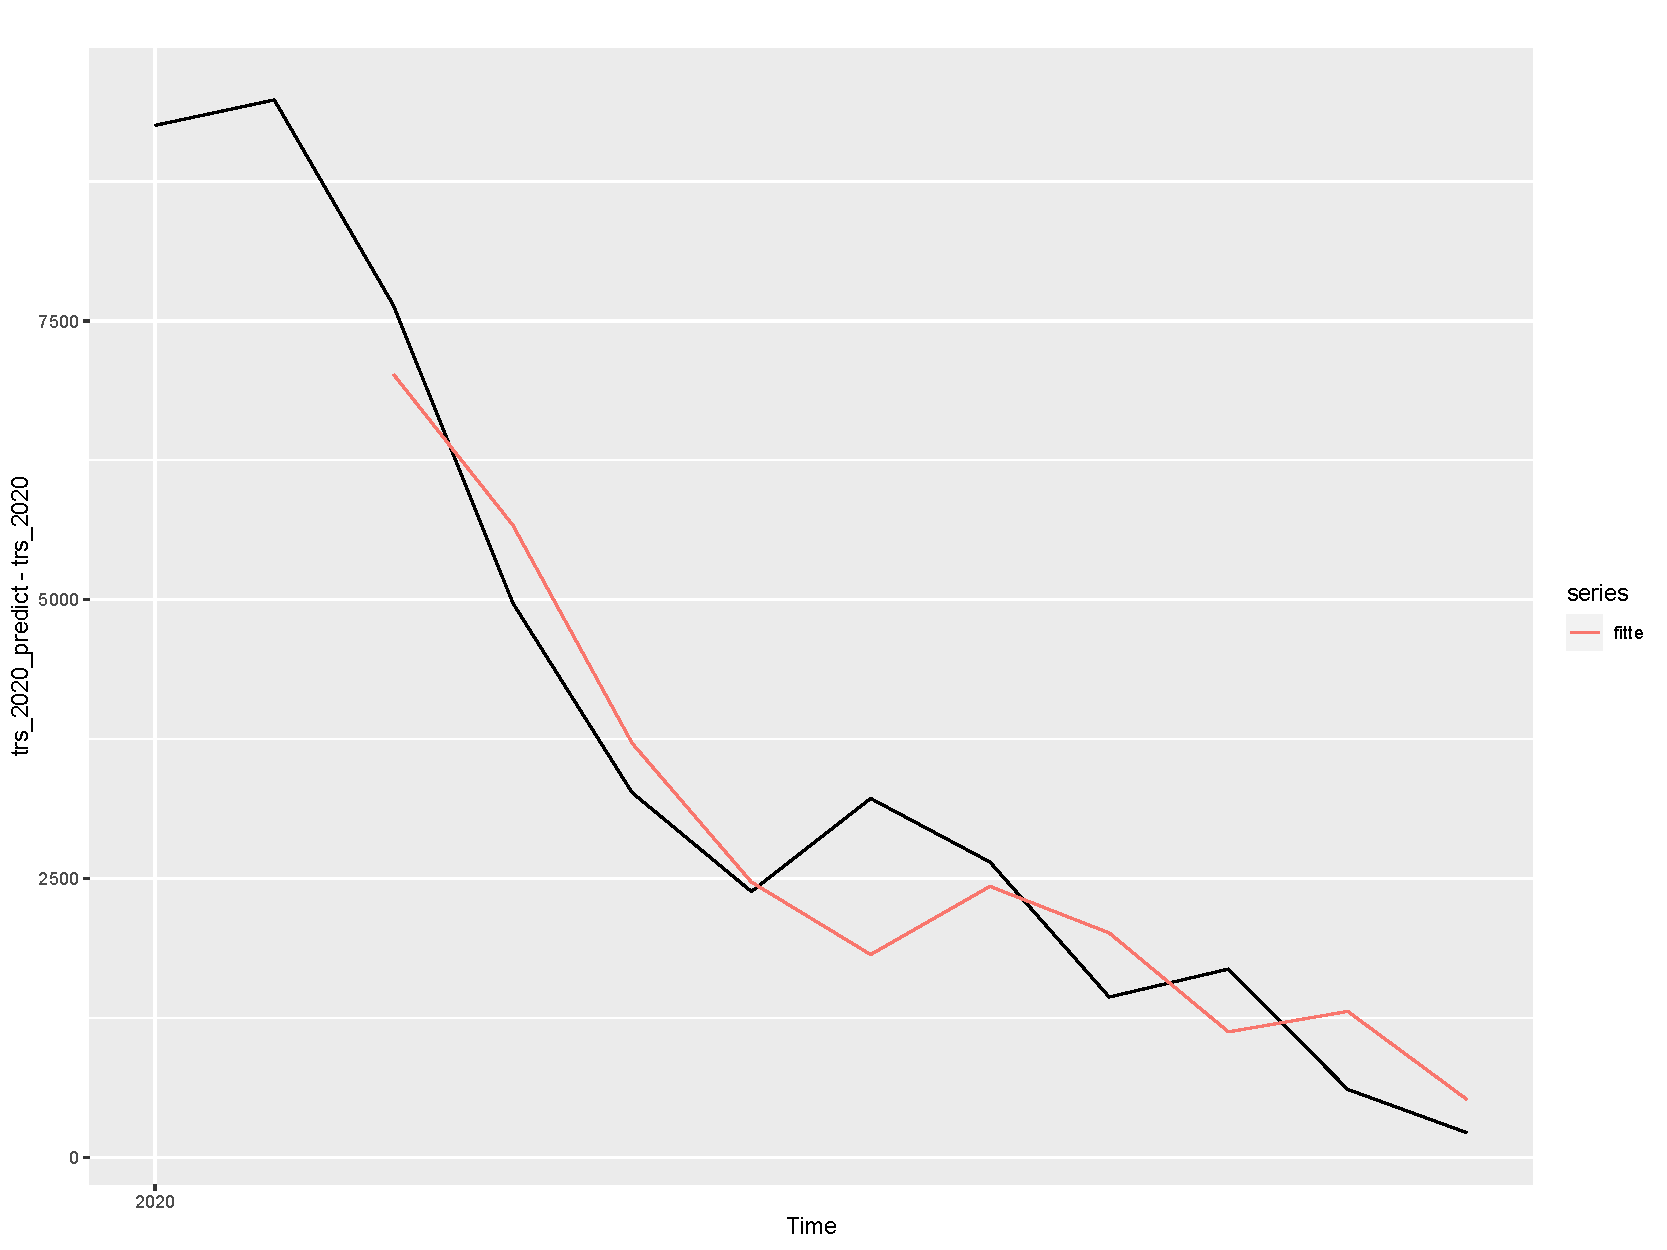
\includegraphics[width=1\textwidth]{fitted_loss_2020.pdf} %插入图片,[]中设置图片大小,{}中是图片文件名
      \caption{2020年社会消费品零售总额的损失图(红色为回归结果)} %最终文档中希望显示的图片标题
      \label{fitted_loss_2020} %用于文内引用的标签
    \end{minipage}
    \begin{minipage}[t]{0.48\textwidth}
      \centering %图片居中
      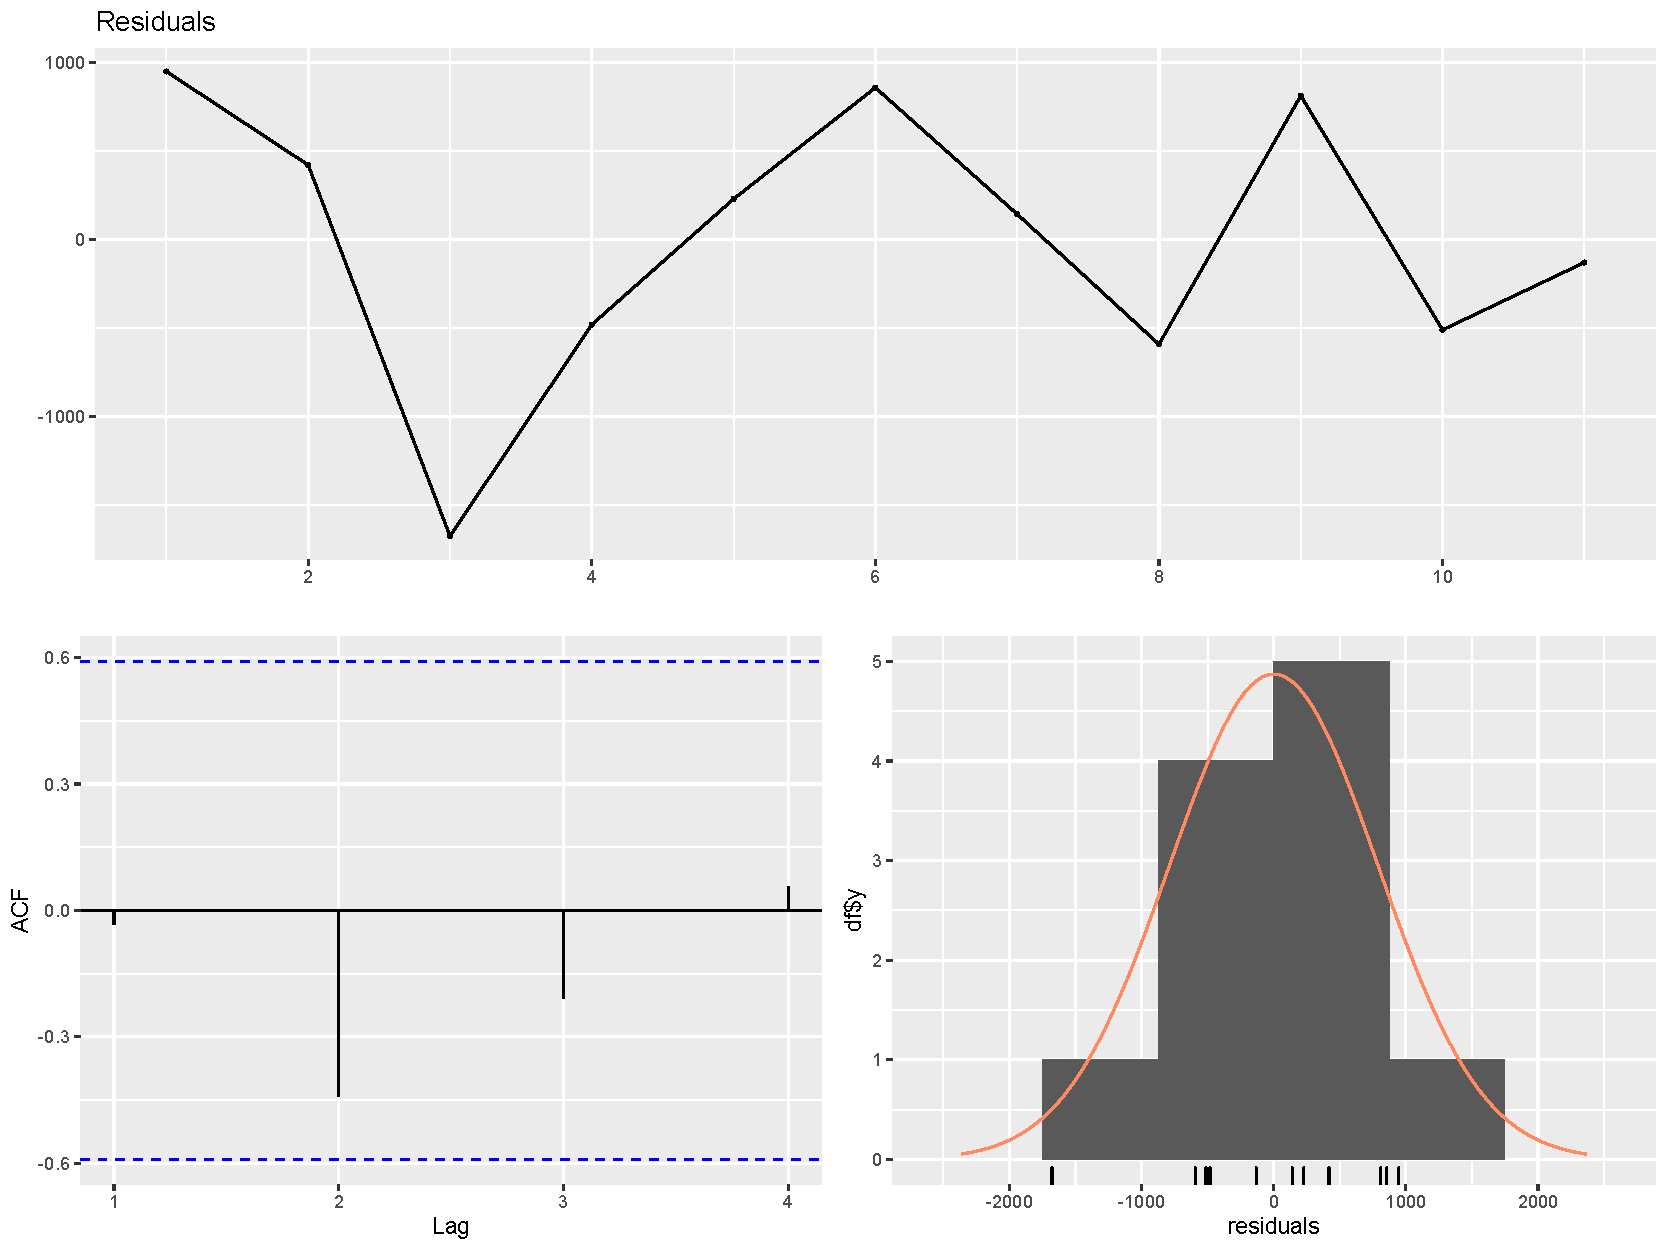
\includegraphics[width=1\textwidth]{loss_model_resi.pdf} %插入图片,[]中设置图片大小,{}中是图片文件名
      \caption{回归结果的残差图} %最终文档中希望显示的图片标题
      \label{loss_model_resi} %用于文内引用的标签
    \end{minipage}
  \end{figure} 
  从残差分布曲线看,残差基本符合正态分布要求, 且通过Ljung-Box检验。
  \subsection{预测2022年的损失}
  假设5月份经济损失有望得到改善,即四月份为损失最严重的时期,那么且疫情不在
  反弹。那么预测从今年三月份开始到年末的社会消费品零售总额损失如下:
  % Table generated by Excel2LaTeX from sheet 'Sheet1'
  \begin{table}[H]
    \centering
    \caption{2022年3月起社会消费品零售总额的损失}
      \begin{tabular}{ccccccccccc}
      月份    & 3     & 4     & 5     & 6     & 7     & 8     & 9     & 10    & 11    & 12 \\
      \hline
      损失    & 3924 & 8587 & 7168 & 6006 & 5054 & 4274 & 3635 & 3111 & 2683 & 2332 \\
      \end{tabular}%
    \label{loss_2020_table}%
  \end{table}%
  绘出社会消费品零售总额的损失如下:
  \begin{figure}[H] %H为当前位置,!htb为忽略美学标准,htbp为浮动图形
    \centering %图片居中
    \begin{minipage}[t]{0.48\textwidth}
      \centering
      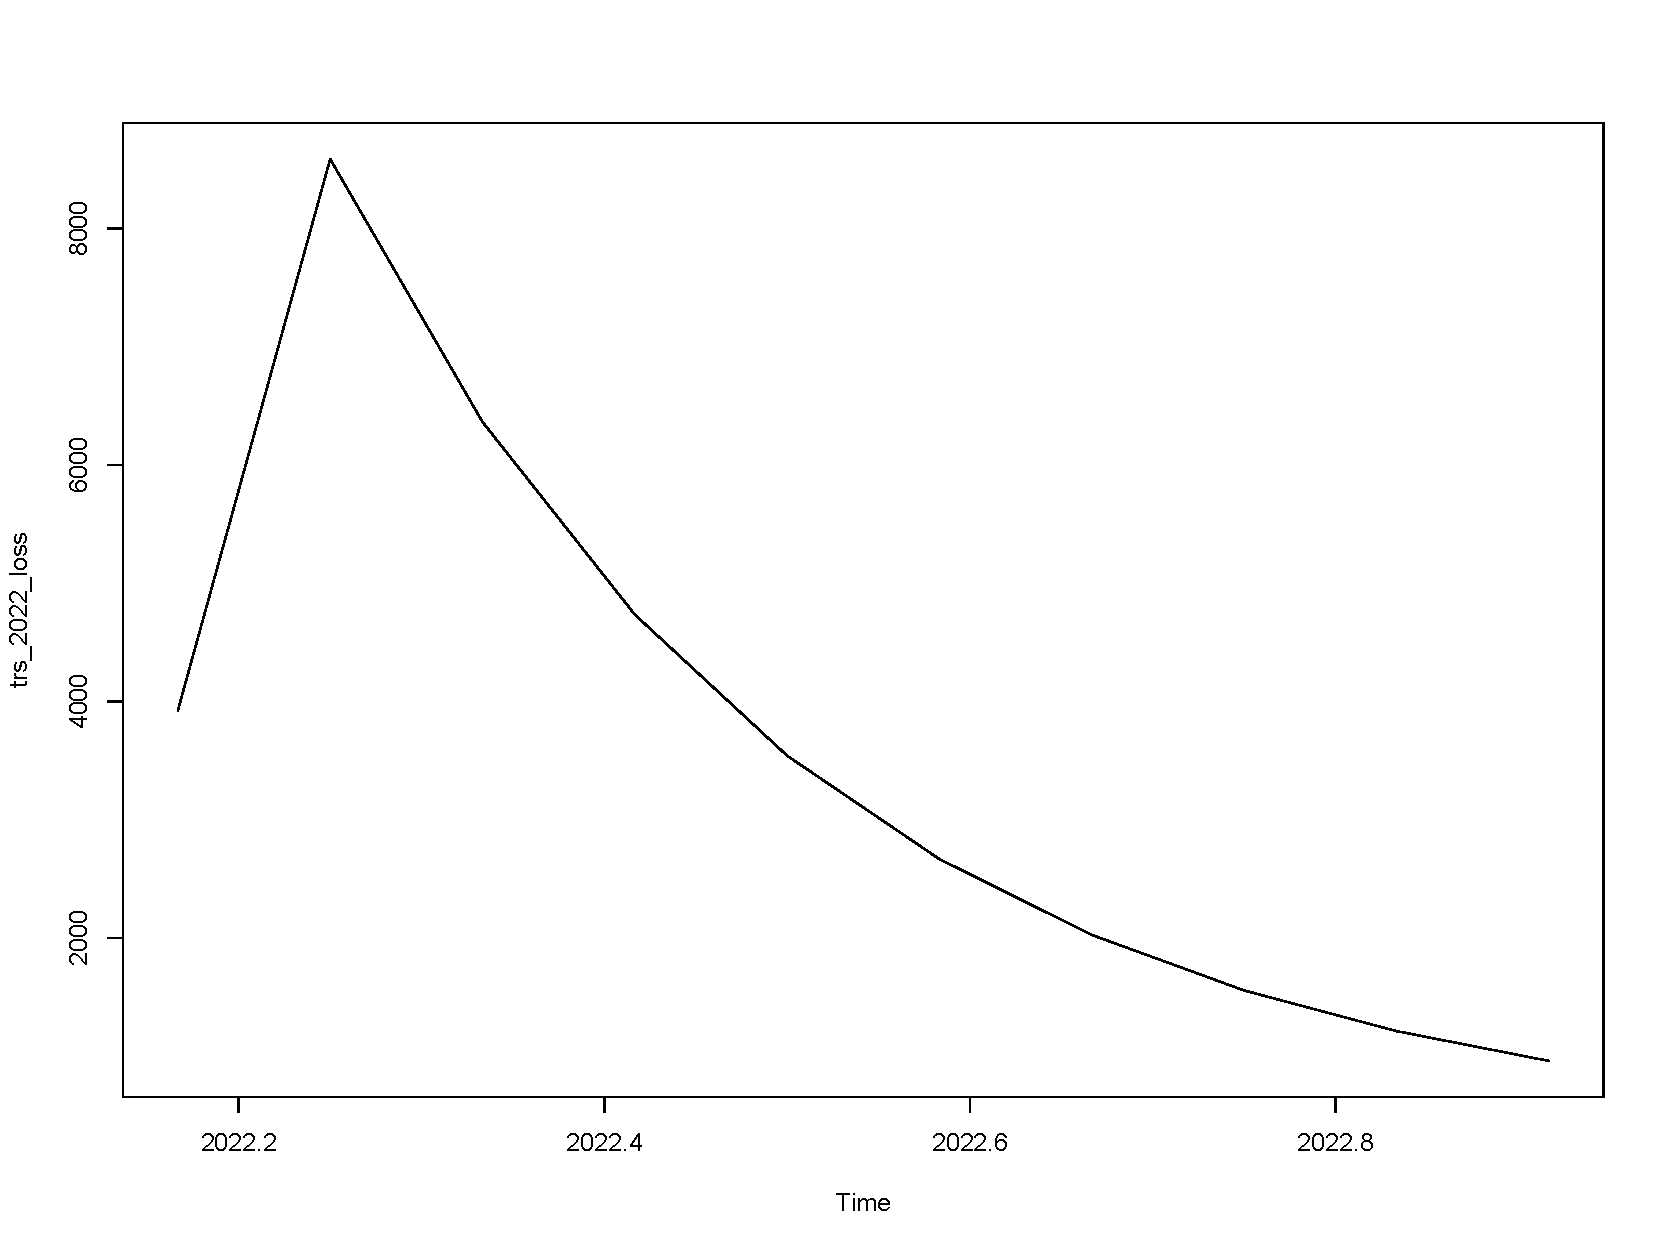
\includegraphics[width=1\textwidth]{loss_2022.pdf} %插入图片,[]中设置图片大小,{}中是图片文件名
      \caption{2022年3月起社会消费品零售总额的损失} %最终文档中希望显示的图片标题
      \label{loss_2022} %用于文内引用的标签
    \end{minipage}
    \begin{minipage}[t]{0.48\textwidth}
      \centering %图片居中
      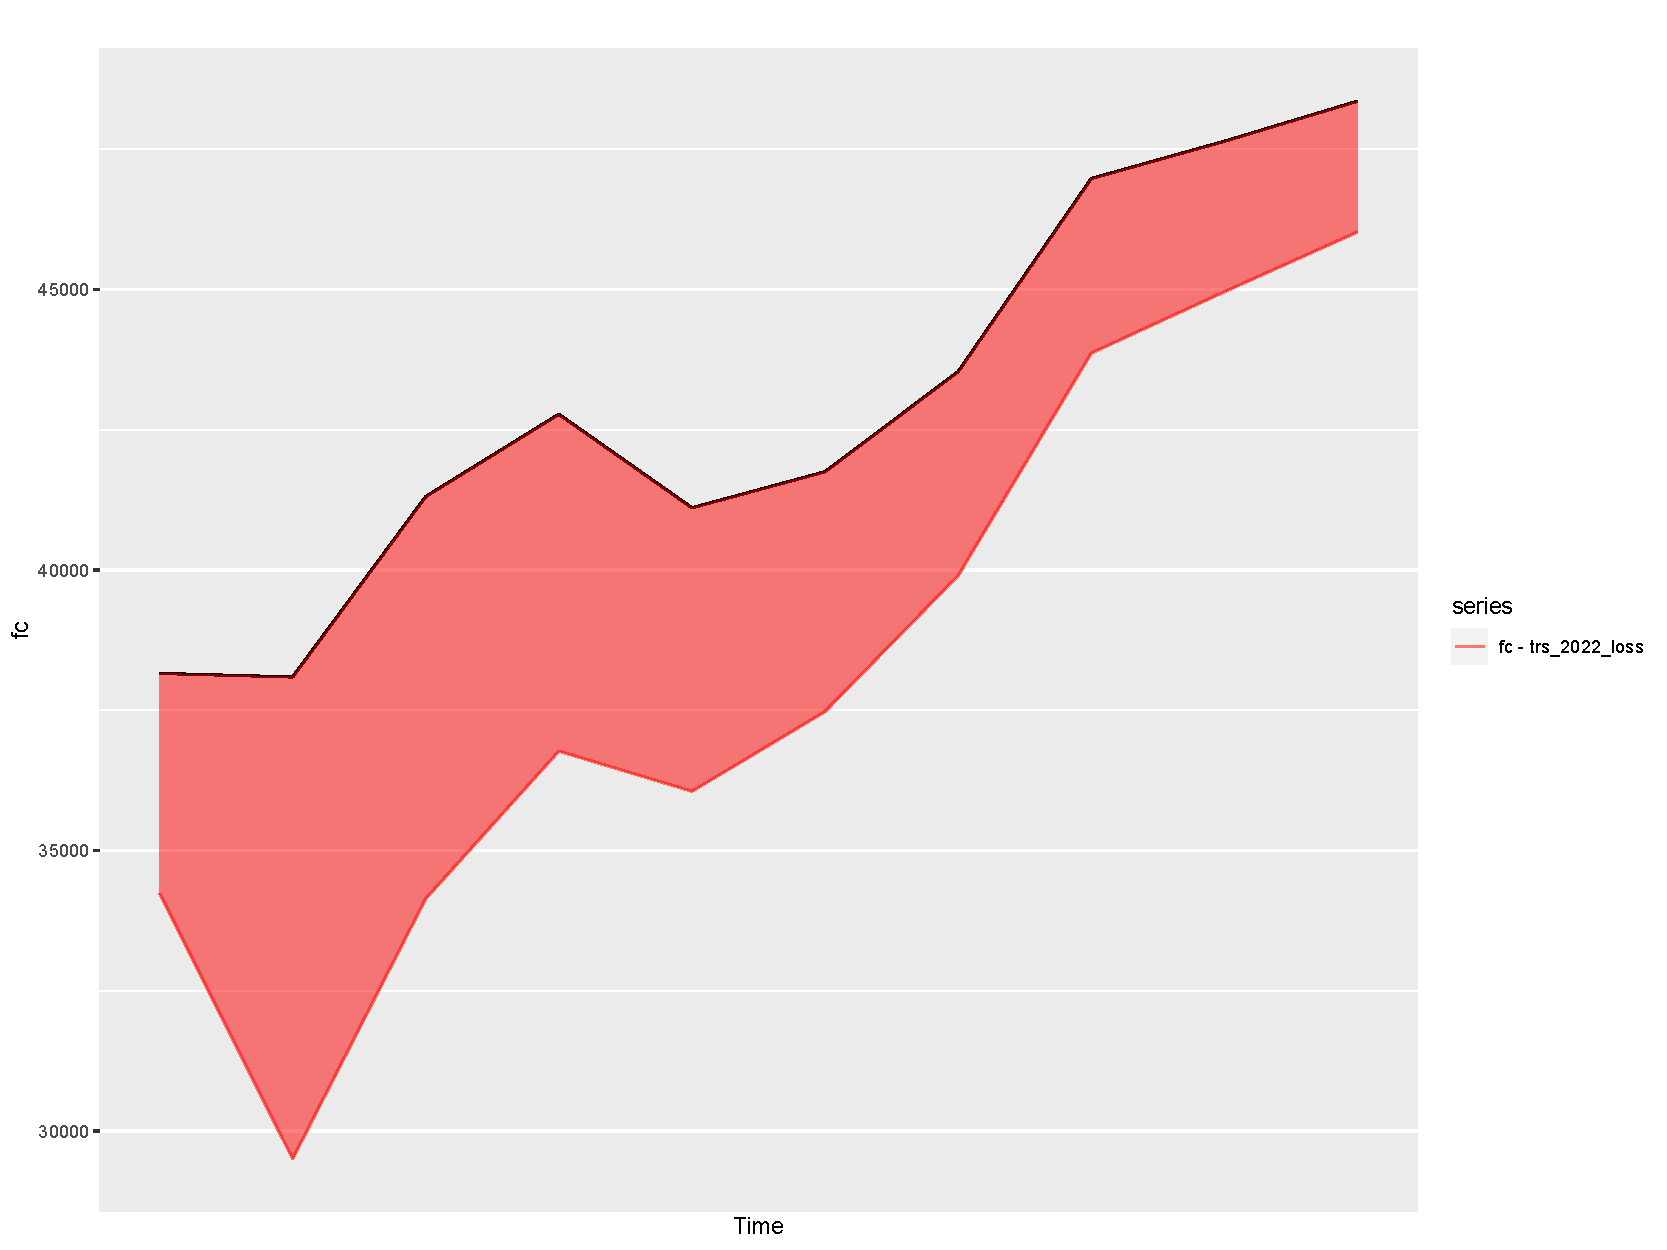
\includegraphics[width=1\textwidth]{compare_2022.pdf} %插入图片,[]中设置图片大小,{}中是图片文件名
      \caption{红色面积为预测损失} %最终文档中希望显示的图片标题
      \label{compare_2022} %用于文内引用的标签
    \end{minipage}
  \end{figure} 
\newpage
\bibliographystyle{gbt7714-numerical}
\bibliography{ref.bib}


\newpage

\begin{appendices}

\section*{}

\textbf{\textcolor[rgb]{0.98,0.00,0.00}{程序一:MATLAB算道路车辆通行能力:}}
\lstinputlisting[language=Matlab]{./code/mcmthesis-matlab1.m}

\section*{}

\textcolor[rgb]{0.98,0.00,0.00}{\textbf{程序二:C++ 求解路网正体影响度:}}
\lstinputlisting[language=C++]{./code/mcmthesis-sudoku.cpp}

\newpage
\def\thesection{A}
\renewcommand{\thetable}{\wuhao A-\arabic{table}}
\setcounter{table}{0}
\section*{数据表格}
\textcolor[rgb]{0.98,0.00,0.00}{\textbf{表格数据:}}

\begin{table*}[h!]
  \centering
  \small
    \caption{附表1数据}
\begin{tabular*}{\linewidth}{p{40pt}<{\centering}p{30pt}<{\centering}
p{30pt}<{\centering}p{40pt}<{\centering}p{50pt}<{\centering}p{70pt}<{\centering}
p{60pt}<{\centering}p{50pt}<{\centering}}
\toprule
样本编号 &  车速 & 车道数  & 侧向 净宽 &  车道宽  &  司机反应时间  & 车辆南止耗时  &  交通量  \\
\midrule
1 & 37 {\color{Blue} } & 2 & 1 & 3 & 0.5 & 1.72 & 1112 \\
2 & 47 & 3 & 2.5 & 3.5 & 0.6 & 2.41 & 1835 \\
3 & 48 & 3 & 2.5 & 3.25 & 1.2 & 2.475 & 2034 \\
4 & 44 & 2 & 2.5 & 3.25 & 1 & 2.26 & 1477 \\
5 & 46 & 3 & 2.5 & 3 & 1.2 & 2.27 & 1648 \\
6 & 53 & 2 & 2.5 & 3.5 & 1.2 & 2.498 & 1952 \\
7 & 54 & 3 & 3.5 & 3.5 & 2 & 2.5 & 2249 \\
8 & 59 & 3 & 3.5 & 3.5 & 0.7 & 2.634 & 1893 \\
9 & 59 & 3 & 3.5 & 3.25 & 0.2 & 2.642 & 2245 \\
10 & 48 & 3 & 2.5 & 3.25 & 0.3 & 2.46 & 2035 \\
11 & 50 & 3 & 4.5 & 3.5 & 0.3 & 2.52 & 2318 \\
12 & 56 & 3 & 3.5 & 3.25 & 0.9 & 2.617 & 2203 \\
13 & 57 & 2 & 2.5 & 3.5 & 0.8 & 2.625 & 2034 \\
14 & 58 & 2 & 2.5 & 3 & 0.6 & 2.641 & 2178 \\
15 & 68 & 4 & 3.5 & 3.25 & 0.9 & 3.05 & 2468 \\
16 & 59 & 3 & 4.5 & 3.75 & 0.6 & 2.975 & 2406 \\
17 & 75 & 4 & 4.5 & 3.75 & 0.7 & 3.15 & 2648 \\
18 & 22 & 1 & 1 & 3 & 1.1 & 1.45 & 800 \\
19 & 27 & 4 & 0.5 & 3 & 0.6 & 1.5 & 903 \\
20 & 75 & 1 & 2.5 & 3.5 & 0.6 & 1.46 & 1010 \\
21 & 76 & 1 & 3.5 & 3.5 & 0.2 & 1.63 & 1069 \\
22 & 46 & 2 & 1.5 & 3.25 & 1.9 & 2.3 & 1682 \\
23 & 46 & 2 & 2.5 & 3.25 & 1 & 2.32 & 1734 \\
24 & 46 & 2 & 2.5 & 3.75 & 0.2 & 2.4 & 1826 \\
25 & 47 & 3 & 2.5 & 3.25 & 1.2 & 2.37 & 1625 \\
26 & 77 & 3 & 4.5 & 3.5 & 0.2 & 2.475 & 2148 \\
27 & 48 & 3 & 4.5 & 3.25 & 0.3 & 2.47 & 2278 \\
28 & 80 & 3 & 2.5 & 3.5 & 0.5 & 2.58 & 2177 \\
29 & 66 & 2 & 3.5 & 3.5 & 1 & 2.72 & 2249 \\
30 & 67 & 4 & 3.5 & 3.75 & 0.9 & 2.975 & 2484 \\
31 & 25 & 3 & 1.5 & 3.5 & 0.6 & 1.3 & 846 \\
32 & 34 & 2 & 4.5 & 3.5 & 0.8 & 1.52 & 1152 \\
33 & 47 & 3 & 2.5 & 3.25 & 0.3 & 2.42 & 1753 \\
34 & 48 & 4 & 2.5 & 3.75 & 0.3 & 2.34 & 1924 \\
35 & 79 & 3 & 2.5 & 3.25 & 1.1 & 2.53 & 2159 \\
36 & 55 & 3 & 0.5 & 3.5 & 0.9 & 2.62 & 1568 \\
37 & 78 & 2 & 1 & 3.5 & 0.9 & 2.618 & 2148 \\
38 & 59 & 3 & 1 & 3.5 & 1 & 2.64 & 2272 \\
39 & 19 & 1 & 0 & 3 & 1.2 & 1.4 & 513 \\
40 & 19 & 2 & 2.5 & 3.25 & 1 & 1.35 & 810 \\
41 & 37 & 2 & 2.5 & 3 & 1.2 & 1.49 & 1102 \\
42 & 45 & 2 & 2.5 & 3.5 & 0.8 & 2.28 & 1525 \\
\bottomrule
  \end{tabular*}
  \label{Ap1}
\end{table*}

\newpage

\begin{table*}[h!]
  \centering
  \small
  \caption{小区开放前VISSIM正常行驶仿真数据记录表1}
\begin{tabular*}{\linewidth}{p{40pt}<{\centering}p{30pt}<{\centering}
p{30pt}<{\centering}p{40pt}<{\centering}p{50pt}<{\centering}p{70pt}<{\centering}
p{60pt}<{\centering}p{50pt}<{\centering}}
\toprule
样本编号 &  车速 & 车道数  & 侧向 净宽 &  车道宽  &  司机反应时间  & 车辆南止耗时  &  交通量  \\
\midrule
47 & 67 & 1 & 0.5 & 3.75 & 0.2 & 2.83 & 2249 \\
48 & 67 & 4 & 3.5 & 3.25 & 0.6 & 2.815 & 2463 \\
49 & 75 & 2 & 3.5 & 3.5 & 0.6 & 3.21 & 2748 \\
50 & 34 & 2 & 1.5 & 3 & 1 & 1.48 & 957 \\
51 & 39 & 2 & 2.5 & 3.5 & 0.8 & 1.97 & 1364 \\
52 & 40 & 3 & 2.5 & 3.25 & 0.5 & 2 & 1359 \\
53 & 50 & 3 & 2.5 & 3.5 & 1 & 2.51 & 2264 \\
54 & 55 & 2 & 3.5 & 3.25 & 1.2 & 2.6 & 1978 \\
55 & 55 & 3 & 3.5 & 3.5 & 0.6 & 2.61 & 2218 \\
56 & 59 & 3 & 0.5 & 3 & 0.2 & 2.638 & 1974 \\
57 & 63 & 4 & 2.5 & 3.5 & 1.1 & 2.78 & 2384 \\
58 & 67 & 3 & 2.5 & 3.75 & 0.8 & 2.83 & 2384 \\
59 & 75 & 3 & 4.5 & 3.5 & 0.3 & 3.2 & 2801 \\
60 & 77 & 2 & 4.5 & 3.5 & 0.2 & 3.18 & 2845 \\
61 & 23 & 1 & 0 & 3 & 0.5 & 1.44 & 458 \\
62 & 75 & 2 & 1 & 3 & 0.2 & 1.625 & 1065 \\
63 & 46 & 2 & 2.5 & 3.5 & 1 & 2.43 & 1752 \\
64 & 61 & 2 & 0.5 & 3 & 1.2 & 2.71 & 1890 \\
65 & 36 & 3 & 2.5 & 3.5 & 1 & 1.67 & 1233 \\
66 & 38 & 2 & 3.5 & 3 & 1.7 & 1.9 & 1246 \\
67 & 55 & 1 & 0.5 & 3.5 & 0.3 & 2.615 & 1763 \\
68 & 74 & 2 & 1.5 & 3.75 & 0.7 & 3.05 & 2349 \\
69 & 79 & 4 & 2.5 & 3.75 & 0.4 & 3.17 & 2694 \\
70 & 38 & 2 & 3.5 & 3 & 1.1 & 1.86 & 1343 \\
71 & 61 & 3 & 1.5 & 3.25 & 0.3 & 2.68 & 2006 \\
72 & 79 & 3 & 3.5 & 3.5 & 2.1 & 3.48 & 2948 \\
73 & 27 & 2 & 1 & 3.75 & 0.8 & 1.48 & 928 \\
74 & 28 & 1 & 1 & 3 & 0.9 & 1.47 & 947 \\
75 & 34 & 2 & 1 & 3 & 0.3 & 1.49 & 998 \\
76 & 44 & 3 & 2.5 & 3.25 & 0.3 & 2.24 & 1520 \\
77 & 78 & 3 & 4.5 & 3.5 & 0.7 & 3.09 & 2648 \\
78 & 73 & 3 & 3.5 & 3.5 & 1.2 & 3.19 & 2741 \\
80 & 37 & 4 & 1 & 3 & 1.7 & 1.87 & 1265 \\
81 & 37 & 2 & 3.5 & 3.5 & 1.5 & 1.84 & 1325 \\
82 & 38 & 2 & 2.5 & 3 & 1.2 & 1.95 & 1233 \\
83 & 38 & 2 & 1 & 3 & 2.1 & 1.97 & 1249 \\
84 & 40 & 2 & 1.5 & 3 & 0.4 & 2.12 & 1366 \\
85 & 42 & 3 & 4.5 & 3.75 & 0.4 & 2.16 & 1638 \\
86 & 40 & 3 & 1.5 & 3.25 & 0.8 & 2.43 & 1384 \\
87 & 41 & 3 & 1.5 & 3.5 & 1.1 & 2.05 & 1434 \\
88 & 78 & 3 & 4.5 & 3.75 & 1.4 & 3.42 & 3048 \\
89 & 41 & 4 & 1.5 & 3.75 & 0.8 & 2.15 & 1566 \\
90 & 42 & 2 & 4.5 & 3.25 & 1.8 & 2.2 & 1466 \\
91 & 44 & 2 & 2.5 & 3 & 1.2 & 2.24 & 1475 \\
92 & 75 & 4 & 4.5 & 3.75 & 1.8 & 3.25 & 2801 \\
93 & 37 & 4 & 4.5 & 3.75 & 0.2 & 1.5 & 2043 \\
94 & 37 & 2 & 1 & 3 & 2.1 & 1.89 & 1289 \\
95 & 40 & 4 & 2.5 & 3.5 & 0.9 & 2.15 & 1406 \\
\bottomrule
  \end{tabular*}
  \label{Ap2}
\end{table*}



\begin{table*}[h!]
  \centering
  \small
  \caption{小区开放前VISSIM正常行驶仿真数据记录表2}
\begin{tabular*}{\linewidth}{p{40pt}<{\centering}p{30pt}<{\centering}
p{30pt}<{\centering}p{40pt}<{\centering}p{50pt}<{\centering}p{70pt}<{\centering}
p{60pt}<{\centering}p{50pt}<{\centering}}
\toprule
样本编号 &  车速 & 车道数  & 侧向 净宽 &  车道宽  &  司机反应时间  & 车辆南止耗时  &  交通量  \\
\midrule
47 & 67 & 1 & 0.5 & 3.75 & 0.2 & 2.83 & 2249 \\
48 & 67 & 4 & 3.5 & 3.25 & 0.6 & 2.815 & 2463 \\
49 & 75 & 2 & 3.5 & 3.5 & 0.6 & 3.21 & 2748 \\
50 & 34 & 2 & 1.5 & 3 & 1 & 1.48 & 957 \\
51 & 39 & 2 & 2.5 & 3.5 & 0.8 & 1.97 & 1364 \\
52 & 40 & 3 & 2.5 & 3.25 & 0.5 & 2 & 1359 \\
53 & 50 & 3 & 2.5 & 3.5 & 1 & 2.51 & 2264 \\
54 & 55 & 2 & 3.5 & 3.25 & 1.2 & 2.6 & 1978 \\
55 & 55 & 3 & 3.5 & 3.5 & 0.6 & 2.61 & 2218 \\
56 & 59 & 3 & 0.5 & 3 & 0.2 & 2.638 & 1974 \\
57 & 63 & 4 & 2.5 & 3.5 & 1.1 & 2.78 & 2384 \\
58 & 67 & 3 & 2.5 & 3.75 & 0.8 & 2.83 & 2384 \\
59 & 75 & 3 & 4.5 & 3.5 & 0.3 & 3.2 & 2801 \\
60 & 77 & 2 & 4.5 & 3.5 & 0.2 & 3.18 & 2845 \\
61 & 23 & 1 & 0 & 3 & 0.5 & 1.44 & 458 \\
62 & 75 & 2 & 1 & 3 & 0.2 & 1.625 & 1065 \\
63 & 46 & 2 & 2.5 & 3.5 & 1 & 2.43 & 1752 \\
64 & 61 & 2 & 0.5 & 3 & 1.2 & 2.71 & 1890 \\
65 & 36 & 3 & 2.5 & 3.5 & 1 & 1.67 & 1233 \\
66 & 38 & 2 & 3.5 & 3 & 1.7 & 1.9 & 1246 \\
67 & 55 & 1 & 0.5 & 3.5 & 0.3 & 2.615 & 1763 \\
68 & 74 & 2 & 1.5 & 3.75 & 0.7 & 3.05 & 2349 \\
69 & 79 & 4 & 2.5 & 3.75 & 0.4 & 3.17 & 2694 \\
70 & 38 & 2 & 3.5 & 3 & 1.1 & 1.86 & 1343 \\
71 & 61 & 3 & 1.5 & 3.25 & 0.3 & 2.68 & 2006 \\
72 & 79 & 3 & 3.5 & 3.5 & 2.1 & 3.48 & 2948 \\
73 & 27 & 2 & 1 & 3.75 & 0.8 & 1.48 & 928 \\
74 & 28 & 1 & 1 & 3 & 0.9 & 1.47 & 947 \\
75 & 34 & 2 & 1 & 3 & 0.3 & 1.49 & 998 \\
76 & 44 & 3 & 2.5 & 3.25 & 0.3 & 2.24 & 1520 \\
77 & 78 & 3 & 4.5 & 3.5 & 0.7 & 3.09 & 2648 \\
78 & 73 & 3 & 3.5 & 3.5 & 1.2 & 3.19 & 2741 \\
80 & 37 & 4 & 1 & 3 & 1.7 & 1.87 & 1265 \\
81 & 37 & 2 & 3.5 & 3.5 & 1.5 & 1.84 & 1325 \\
82 & 38 & 2 & 2.5 & 3 & 1.2 & 1.95 & 1233 \\
83 & 38 & 2 & 1 & 3 & 2.1 & 1.97 & 1249 \\
84 & 40 & 2 & 1.5 & 3 & 0.4 & 2.12 & 1366 \\
85 & 42 & 3 & 4.5 & 3.75 & 0.4 & 2.16 & 1638 \\
86 & 40 & 3 & 1.5 & 3.25 & 0.8 & 2.43 & 1384 \\
87 & 41 & 3 & 1.5 & 3.5 & 1.1 & 2.05 & 1434 \\
88 & 78 & 3 & 4.5 & 3.75 & 1.4 & 3.42 & 3048 \\
89 & 41 & 4 & 1.5 & 3.75 & 0.8 & 2.15 & 1566 \\
90 & 42 & 2 & 4.5 & 3.25 & 1.8 & 2.2 & 1466 \\
91 & 44 & 2 & 2.5 & 3 & 1.2 & 2.24 & 1475 \\
92 & 75 & 4 & 4.5 & 3.75 & 1.8 & 3.25 & 2801 \\
93 & 37 & 4 & 4.5 & 3.75 & 0.2 & 1.5 & 2043 \\
94 & 37 & 2 & 1 & 3 & 2.1 & 1.89 & 1289 \\
95 & 40 & 4 & 2.5 & 3.5 & 0.9 & 2.15 & 1406 \\
\bottomrule
  \end{tabular*}
  \label{Ap3}
\end{table*}

\begin{table*}[h!]
  \centering
  \small
  \caption{小区开放前VISSIM正常行驶仿真数据记录表3}
\begin{tabular*}{\linewidth}{p{50pt}<{\centering}p{50pt}<{\centering}
p{60pt}<{\centering}p{60pt}<{\centering}p{60pt}<{\centering}p{70pt}<{\centering}}
\toprule
 数据P.C. & 时间(进入) & 时间(离开) & 车辆编号& 速度(m/s) & 车辆长度(m) \\
\midrule
1 & 9.34 & -1 & 4 & 14.7 & 4.76 \\
1 & -1 & 9.67 & 4 & 14.7 & 4.76 \\
7 & 19.34 & -1 & 3 & 14.7 & 4.76 \\
7 & -1 & 19.66 & 3 & 14.8 & 4.76 \\
6 & 20.35 & -1 & 4 & 14 & 4.76 \\
6 & -1 & 20.69 & 4 & 14 & 4.76 \\
1 & 21.49 & -1 & 11 & 14.8 & 4.61 \\
2 & 21.43 & -1 & 5 & 15.9 & 4.55 \\
1 & -1 & 21.8 & 11 & 14.9 & 4.61 \\
2 & -1 & 21.72 & 5 & 15.9 & 4.55 \\
5 & 22.36 & -1 & 6 & 15.4 & 4.61 \\
5 & -1 & 22.66 & 6 & 15.4 & 4.61 \\
2 & 25.81 & -1 & 7 & 13.8 & 4.11 \\
2 & -1 & 26.11 & 7 & 13.8 & 4.11 \\
2 & 27.19 & -1 & 8 & 14.1 & 10.21 \\
2 & -1 & 27.92 & 8 & 14.2 & 10.21 \\
7 & 29.24 & -1 & 10 & 15.1 & 4.76 \\
7 & -1 & 29.55 & 10 & 15.1 & 4.76 \\
6 & 32.23 & -1 & 11 & 14.5 & 4.61 \\
6 & -1 & 32.55 & 11 & 14.6 & 4.61 \\
5 & 35.38 & -1 & 12 & 14.8 & 4.55 \\
5 & -1 & 35.68 & 12 & 14.9 & 4.55 \\
7 & 36.42 & -1 & 13 & 14.5 & 4.55 \\
7 & -1 & 36.73 & 13 & 14.5 & 4.55 \\
1 & 38.87 & -1 & 16 & 15.4 & 4.61 \\
1 & -1 & 39.16 & 16 & 15.4 & 4.61 \\
6 & 49.09 & -1 & 16 & 15.1 & 4.61 \\
6 & -1 & 49.4 & 16 & 15.1 & 4.61 \\
1 & 49.91 & -1 & 24 & 15.1 & 4.55 \\
1 & -1 & 50.21 & 24 & 15.2 & 4.55 \\
5 & 50.59 & -1 & 17 & 15.3 & 4.55 \\
5 & -1 & 50.89 & 17 & 15.3 & 4.55 \\
3 & 56.27 & -1 & 14 & 15.8 & 4.76 \\
3 & -1 & 56.57 & 14 & 15.9 & 4.76 \\
7 & 57.12 & -1 & 23 & 15.9 & 4.76 \\
7 & -1 & 57.42 & 23 & 15.8 & 4.76 \\
6 & 60.56 & -1 & 24 & 14.6 & 4.55 \\
6 & -1 & 60.87 & 24 & 14.7 & 4.55 \\
3 & 63.02 & -1 & 18 & 15.1 & 4.11 \\
3 & -1 & 63.29 & 18 & 15.1 & 4.11 \\
3 & 66.53 & -1 & 15 & 15 & 4.11 \\
1 & 66.65 & -1 & 33 & 15 & 4.4 \\
1 & -1 & 66.94 & 33 & 15.1 & 4.4 \\
3 & -1 & 66.8 & 15 & 14.9 & 4.11 \\
5 & 67.35 & -1 & 28 & 14.7 & 4.76 \\
5 & -1 & 67.68 & 28 & 14.7 & 4.76 \\
\bottomrule
  \end{tabular*}
  \label{Ap3}
\end{table*}

\newpage

\begin{table*}[h!]
  \centering
  \small
  \caption{小区开放前VISSIM正常行驶仿真数据记录表1}
\begin{tabular*}{\linewidth}{p{50pt}<{\centering}p{50pt}<{\centering}
p{60pt}<{\centering}p{60pt}<{\centering}p{60pt}<{\centering}p{70pt}<{\centering}}
\toprule
 数据P.C. & 时间(进入) & 时间(离开) & 车辆编号& 速度(m/s) & 车辆长度(m) \\
\midrule
5 & -1 & 80.44 & 35 & 15 & 4.55 \\
7 & 84.64 & -1 & 37 & 14.5 & 10.21 \\
7 & -1 & 85.35 & 37 & 14.4 & 10.21 \\
3 & 89.77 & -1 & 31 & 14.7 & 4.76 \\
3 & -1 & 90.09 & 31 & 14.8 & 4.76 \\
2 & 90.42 & -1 & 32 & 15.2 & 4.11 \\
2 & -1 & 90.69 & 32 & 15.2 & 4.11 \\
1 & 90.84 & -1 & 40 & 1.7 & 11.54 \\
3 & 93.85 & -1 & 34 & 13.9 & 4.76 \\
3 & -1 & 94.19 & 34 & 14 & 4.76 \\
1 & -1 & 98.34 & 40 & 1.8 & 11.54 \\
1 & 101.18 & -1 & 44 & 3.5 & 4.4 \\
2 & 101.41 & -1 & 29 & 14.6 & 4.61 \\
2 & -1 & 101.73 & 29 & 14.5 & 4.61 \\
1 & -1 & 101.8 & 44 & 4.3 & 4.4 \\
3 & 103.39 & -1 & 36 & 14.5 & 4.76 \\
3 & -1 & 103.72 & 36 & 1.5 & 4.76 \\
2 & 109.33 & -1 & 39 & 15.7 & 4.76 \\
2 & -1 & 109.63 & 39 & 15.7 & 4.76 \\
1 & 113.78 & -1 & 52 & 3.3 & 4.11 \\
1 & -1 & 114.75 & 52 & 5.6 & 4.11 \\
6 & 116.66 & -1 & 46 & 15 & 4.4 \\
6 & -1 & 116.96 & 46 & 15 & 4.4 \\
4 & 117.67 & -1 & 1 & 2 & 0.44 \\
4 & -1 & 117.89 & 1 & 2 & 0.44 \\
6 & 119.37 & -1 & 44 & 14.2 & 4.4 \\
6 & -1 & 119.68 & 44 & 14.1 & 4.4 \\
1 & 127.94 & -1 & 56 & 1.2 & 0.34 \\
1 & -1 & 128.22 & 56 & 1.2 & 0.34 \\
3 & 128.54 & -1 & 45 & 12.7 & 4.34 \\
3 & -1 & 128.87 & 45 & 13 & 4.34 \\
4 & 128.86 & -1 & 38 & 3.4 & 1.45 \\
4 & -1 & 129.28 & 38 & 3.5 & 1.45 \\
6 & 132.61 & -1 & 52 & 14.2 & 4.11 \\
1 & 132.94 & -1 & 60 & 1.6 & 4.4 \\
1 & 101.18 & -1 & 44 & 3.5 & 4.4 \\
2 & 101.41 & -1 & 29 & 14.6 & 4.61 \\
2 & -1 & 101.73 & 29 & 14.5 & 4.61 \\
1 & -1 & 101.8 & 44 & 4.3 & 4.4 \\
3 & 103.39 & -1 & 36 & 14.5 & 4.76 \\
3 & -1 & 103.72 & 36 & 1.5 & 4.76 \\
2 & 109.33 & -1 & 39 & 15.7 & 4.76 \\
2 & -1 & 109.63 & 39 & 15.7 & 4.76 \\
1 & 113.78 & -1 & 52 & 3.3 & 4.11 \\
1 & -1 & 114.75 & 52 & 5.6 & 4.11 \\
6 & 116.66 & -1 & 46 & 15 & 4.4 \\
\bottomrule
  \end{tabular*}
  \label{Ap4}
\end{table*}



\begin{table*}[h!]
  \centering
  \small
  \caption{小区开放前VISSIM正常行驶仿真数据记录表2}
\begin{tabular*}{\linewidth}{p{50pt}<{\centering}p{50pt}<{\centering}
p{60pt}<{\centering}p{60pt}<{\centering}p{60pt}<{\centering}p{70pt}<{\centering}}
\toprule
 数据P.C. & 时间(进入) & 时间(离开) & 车辆编号& 速度(m/s) & 车辆长度(m) \\
\midrule
1 & 127.94 & -1 & 56 & 1.2 & 0.34 \\
1 & -1 & 128.22 & 56 & 1.2 & 0.34 \\
3 & 128.54 & -1 & 45 & 12.7 & 4.34 \\
3 & -1 & 128.87 & 45 & 13 & 4.34 \\
4 & 128.86 & -1 & 38 & 3.4 & 1.45 \\
4 & -1 & 129.28 & 38 & 3.5 & 1.45 \\
2 & -1 & 90.69 & 32 & 15.2 & 4.11 \\
1 & 90.84 & -1 & 40 & 1.7 & 11.54 \\
3 & 93.85 & -1 & 34 & 13.9 & 4.76 \\
3 & -1 & 94.19 & 34 & 14 & 4.76 \\
1 & -1 & 98.34 & 40 & 1.8 & 11.54 \\
1 & 101.18 & -1 & 44 & 3.5 & 4.4 \\
2 & 101.41 & -1 & 29 & 14.6 & 4.61 \\
2 & -1 & 101.73 & 29 & 14.5 & 4.61 \\
1 & -1 & 101.8 & 44 & 4.3 & 4.4 \\
3 & 103.39 & -1 & 36 & 14.5 & 4.76 \\
3 & -1 & 103.72 & 36 & 1.5 & 4.76 \\
2 & 109.33 & -1 & 39 & 15.7 & 4.76 \\
2 & -1 & 109.63 & 39 & 15.7 & 4.76 \\
1 & 113.78 & -1 & 52 & 3.3 & 4.11 \\
1 & -1 & 114.75 & 52 & 5.6 & 4.11 \\
6 & 116.66 & -1 & 46 & 15 & 4.4 \\
6 & -1 & 116.96 & 46 & 15 & 4.4 \\
4 & 117.67 & -1 & 1 & 2 & 0.44 \\
4 & -1 & 117.89 & 1 & 2 & 0.44 \\
6 & 119.37 & -1 & 44 & 14.2 & 4.4 \\
6 & -1 & 119.68 & 44 & 14.1 & 4.4 \\
1 & 127.94 & -1 & 56 & 1.2 & 0.34 \\
1 & -1 & 128.22 & 56 & 1.2 & 0.34 \\
3 & 128.54 & -1 & 45 & 12.7 & 4.34 \\
3 & -1 & 128.87 & 45 & 13 & 4.34 \\
4 & 128.86 & -1 & 38 & 3.4 & 1.45 \\
4 & -1 & 129.28 & 38 & 3.5 & 1.45 \\
6 & 132.61 & -1 & 52 & 14.2 & 4.11 \\
1 & 132.94 & -1 & 60 & 1.6 & 4.4 \\
1 & 101.18 & -1 & 44 & 3.5 & 4.4 \\
2 & 101.41 & -1 & 29 & 14.6 & 4.61 \\
2 & -1 & 101.73 & 29 & 14.5 & 4.61 \\
1 & -1 & 101.8 & 44 & 4.3 & 4.4 \\
3 & 103.39 & -1 & 36 & 14.5 & 4.76 \\
3 & -1 & 103.72 & 36 & 1.5 & 4.76 \\
2 & -1 & 109.63 & 39 & 15.7 & 4.76 \\
1 & 113.78 & -1 & 52 & 3.3 & 4.11 \\
1 & -1 & 114.75 & 52 & 5.6 & 4.11 \\
6 & 116.66 & -1 & 46 & 15 & 4.4 \\
6 & -1 & 116.96 & 46 & 15 & 4.4 \\
\bottomrule
  \end{tabular*}
  \label{Ap4}
\end{table*}







\end{appendices}
\end{document}
%%
%% This work consists of these files mcmthesis.dtx,
%%                                   figures/ and
%%                                   code/,
%% and the derived files             mcmthesis.cls,
%%                                   mcmthesis-demo.tex,
%%                                   README,
%%                                   LICENSE,
%%                                   mcmthesis.pdf and
%%                                   mcmthesis-demo.pdf.
%%
%% End of file `mcmthesis-demo.tex'.
